%--------------------------------------------------------------
% thesis.tex 
%--------------------------------------------------------------
% - template for the main file of Informatica@Unifi Thesis 
% - based on Classic Thesis Style Copyright (C) 2008 
%   Andr\'e Miede http://www.miede.de   
%--------------------------------------------------------------
\documentclass[titlepage,fleqn,oneside,
	headinclude,12pt,a4paper,footinclude,pdfspacing]{scrbook}%twoside,makeidx,openright
%--------------------------------------------------------------
\usepackage[italian]{babel}
\usepackage[utf8]{inputenc} 
\usepackage[T1]{fontenc} 
\usepackage[square,numbers]{natbib} 
\usepackage[fleqn]{amsmath}
\usepackage{amssymb}
\usepackage{ellipsis}
\usepackage{listings}
\usepackage{subfig}
\usepackage[format=plain,labelformat=simple,labelsep=colon]{caption}
\usepackage{appendix}
\usepackage{siunitx}
\usepackage{lipsum}
\usepackage{dia-classicthesis-ldpkg}
\usepackage[eulerchapternumbers,linedheaders,subfig,beramono,eulermath,
parts,dottedtoc]{classicthesis}
%\usepackage{imakeidx}
\usepackage{wrapfig}
\usepackage[italian,noabbrev]{cleveref}
\usepackage{acronym}
\usepackage{bbding}
%---------------------------------------------------------------
\newcommand{\myItalianTitle}{Analisi di sicurezza di un'applicazione Android\xspace}
\newcommand{\myEnglishTitle}{Titolo inglese\xspace}
\newcommand{\myDegree}{Master di I livello in Cybersecurity\xspace}
\newcommand{\myName}{Candidato: Marco Buracchi\xspace}
\newcommand{\myProf}{Tutor Aziendale: Alessandro Maulà \\ Tutor Accademico: Dr. Gianpiero Costantino\xspace}
\newcommand{\myFaculty}{Dipartimento di Ingegneria dell'Informazione\xspace}
\newcommand{\myUni}{\protect{Università di Pisa}\xspace}
\newcommand{\myLocation}{Pisa\xspace}
\newcommand{\myTime}{Anno Accademico 2018-2019\xspace}
\newcommand{\mycopyright}{
\includegraphics[width=1.5cm]{logo/cc.png} 
	\href{https://creativecommons.org/licenses/by-nc-sa/4.0/}{Creative
		Commons Attribution-NonCommercial-ShareAlike 4.0 International (CC BY-NC-SA 4.0)  }\xspace}

\newcommand{\myfloatalign}{\centering} 

\renewcommand{\lstlistingname}{Codice}% Listing -> Codice
%--------------------------------------------------------------
\newlength{\abcd} % for ab..z string length calculation
% how all the floats will be aligned
\setlength{\extrarowheight}{3pt}	% increase table row height
\captionsetup{format=hang,font=small}
%--------------------------------------------------------------
% Layout setting
%--------------------------------------------------------------
\graphicspath{{img/}}
\usepackage{geometry}
\geometry{
	a4paper,
	ignoremp,
	%bindingoffset = 1cm, 
	textwidth     = 13cm,
	textheight    = 21.5cm,
	%lmargin       = 3.5cm, left margin
	%tmargin       = 4cm	% top margin 
}

\crefname{listing}{codice}{codici}
%---------------------PARAMETERS-------------------------------
\begin{document}
\frenchspacing
\raggedbottom
\pagenumbering{roman}
\pagestyle{plain}

\lstset{
	string=[s]{"}{"},
	stringstyle=\color{blue},
	comment=[l]{:},
	commentstyle=\color{black},
	captionpos=b,
	frame=none
}
%---------------------FRONTMATTER------------------------------
%--------------------------------------------------------------
% titlepage.tex (use thesis.tex as main file)
%--------------------------------------------------------------
\begin{titlepage}
	\begin{center}
   	\large
      \hfill
      \vfill
      \begingroup
         
\includegraphics[scale=0.15]{logo/LOGO}\\
%\left 			\spacedallcaps{\myUni} \\ 
			\myFaculty \\
			\vspace{0.5cm}
			\myDegree \\ 
			Curriculum: \emph{\myCurriculum}\\
			\vspace{0.5cm}
         \vspace{0.5cm}    
         Tesi di Laurea Magistrale 
      \endgroup 
      \vfill 
      \begingroup
      	\color{Maroon}\spacedallcaps{\myItalianTitle} \\ $\ $\\
      	\spacedallcaps{\myEnglishTitle} \\ 	
	\bigskip
      \endgroup
      \spacedlowsmallcaps{\myName}
      \vfill 
      \vfill
      Relatore: Prof. \emph{\myProf}\\
      \vfill
      \vfill
      \myTime
      \vfill                      
	\end{center}        
\end{titlepage}   
%--------------------------------------------------------------
% back titlepage
%--------------------------------------------------------------
   \newpage
	\thispagestyle{empty}
	\hfill
	\vfill
	\noindent\myName: 
	\textit{\myItalianTitle,} 
	\myDegree, \mycopyright, \myUni, \myTime
%--------------------------------------------------------------
% back titlepage end
%--------------------------------------------------------------
\pagestyle{scrheadings}
%---------------------MAINMATTER-------------------------------
\pagenumbering{arabic}
\tableofcontents
%\listoffigures
%\lstlistoflistings
%\listoftables
%\endgroup 
\cleardoublepage
%-----------------CAPITOLI-------------------------------------
\addcontentsline{toc}{chapter}{Introduzione}
\chapter*{Introduzione}
	\markboth{Introduzione}{}
	\lipsum
%	Il mondo moderno è ormai pervaso dalla \emph{crittografia}. Quotidianamente e spesso inconsapevolmente utilizziamo funzioni crittografiche per le normali operazioni della vita quotidiana. Controllare il conto sull'home-banking, scambiarsi messaggi tramite servizi di messaggistica o anche navigare in internet utilizzando il protocollo \acs{HTTPS} sono azioni che svolgiamo ormai con naturalezza. I sistemi moderni rendono trasparente all'utente l'utilizzo di tali tecnologie, ma ciò non vuol dire che esse non esistano.
%	
%	Una \emph{funzione crittografica}\index{Funzione crittografica} è un oggetto matematico astratto che, attraverso l'utilizzo di una chiave, trasforma un dato in input (plaintext) in una sua rappresentazione diversa (ciphertext) il più possibile non riconducibile al dato originale. Questa funzione deve poi essere implementata in un programma che girerà su un \emph{dispositivo crittografico} in un certo ambiente, presentando perciò caratteristiche fisiche peculiari. Esempi di \dispp potrebbero essere smartcard, chiavette \acs{USB}, chip dedicati montati su dispositivi general purpose (smartphone, notebook) o periferiche progettate e costruite apposta per effettuare questo unico compito.
%	
%	In passato si guardava ad un \disps semplicemente come una black-box che riceveva un plaintext e restituiva un ciphertext (encryption) e viceversa (decryption) come in \cref{fig:blackbox}. Gli attacchi erano basati sulla conoscenza del ciphertext (ciphertext-only attacks) o di alcune coppie di entrambi (known plaintext attacks). Con l'accesso al meccanismo di encryption o di decryption, anche solo temporaneo, si possono attuare anche altri due tipi di attacchi (rispettivamente chosen-plaintext e chosen-ciphertext)\cite{dispenseCS}.
%	
%	\begin{figure}
%		\begin{center}
%			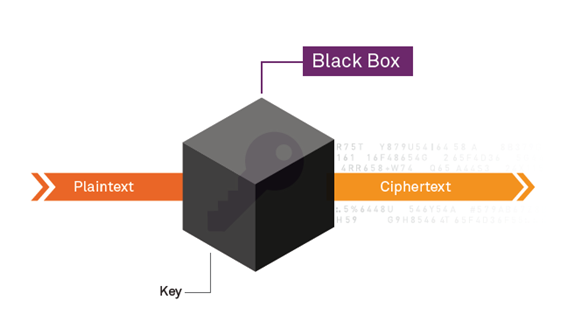
\includegraphics[width=.8\textwidth]{blackbox}
%			\caption{black-box encryption}
%			\label{fig:blackbox}
%		\end{center}
%	\end{figure}
%	
%	Al giorno d'oggi si è consapevoli del fatto che un \disps ha spesso altri input oltre al plaintext e altri output oltre al ciphertext. Gli input differenti dal plaintext possono essere le interazioni col mondo esterno come modifiche al voltaggio della corrente, condizioni atmosferiche particolari o sollecitazioni fisiche. Il nostro interesse sarà però focalizzato sulle informazioni (facilmente misurabili) che vengono lasciate trapelare dai dispositivi stessi oltre al ciphertext come ad esempio il tempo di esecuzione di un programma, le radiazioni emesse, suoni, luci e quant'altro chiamate \emph{side-channel informations}\index{Side-channel informations}.
%	 
%	 Il resto della tesi è organizzata nel seguente modo:
%	 \begin{itemize}
%	 	\item nel capitolo $1$, data l'eterogeneità della letteratura su questo argomento, abbiamo definito una classificazione dei side-channel attacks e abbiamo presentato una panoramica dello stato dell'arte.
%	 	\item nel capitolo $2$ abbiamo focalizzato la nostra attenzione sulla categoria dei \emph{timing attacks}, una particolare tipologia di side-channel attack basato sull'osservazione del tempo di esecuzione di un programma. Partendo da alcuni timing attack reali eseguiti su particolari funzioni crittografiche, abbiamo ottenuto una generalizzazione applicabile a qualunque attacco di questo tipo. Abbiamo anche implementato una piccola funzione crittografica ed effettuato una validazione sperimentale di questa nostra generalizzazione.
%	 	\item nel capitolo $3$ presentiamo i cache attacks, attacchi side-channel (prevalentemente di tipo timing) che colpiscono la memoria cache dei processori.
%	 	\item nel capitolo $4$ abbiamo presentato approfonditamente il progetto \emph{SPECTRE}, la principale famiglia di timing attacks sulle cache, che affligge tutti i recenti processori AMD, ARM e Intel.
%	 	\item nel capitolo $5$ descriviamo infine \ac{SPARK}, l'attacco da noi creato. Questo attacco, basato sui concetti del progetto SPECTRE, è in grado di ottenere dati protetti da password senza la conoscenza di quest'ultima.
%	 \end{itemize}    

\chapter{Analisi statiche}
In questa sezione sono presentati gli strumenti utilizzati per effettuare le scansioni statiche. I risultati verranno aggregati e commentati insieme a quelli delle analisi dinamiche nella sezione $3$.

%----------------------------------------------------%
%--------------------- MARA -------------------------%
%----------------------------------------------------%

\section{MARA Framework}

\begin{figure}[h]
	\centering 
	\fbox{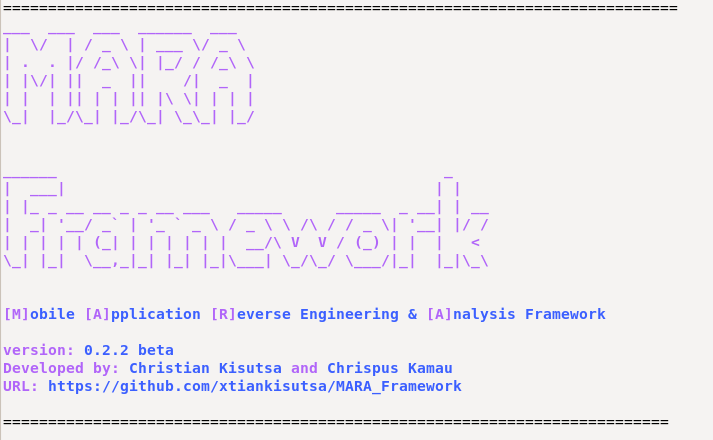
\includegraphics[width=.5\textwidth]{mara/MARABN}}
	\caption{MARA Framework}
	\label{fig:mara} 
\end{figure}

Il primo strumento utilizzato è stato \ac{MARA} Framework(figura \ref{fig:mara})\cite{MARA}. Questo framework unisce vari strumenti comunemente utilizzati per effettuare reverse engineering ed analisi di applicazioni mobili. MARA è particolarmente focalizzato sulle minacce indicate dalla OWASP Foundation\cite{OWASP} come più diffuse e pericolose.
Le operazioni che permette di fare sono le seguenti:
\begin{itemize}
	\item Reverse engineering dell'apk
	\item De-offuscamento dell'apk
	\item Analisi dell'apk
	\item Analisi del manifest
	\item Analisi del codice sorgente
\end{itemize}

L'esecuzione dell'analisi di MARA sull'apk si compone di vari passi (figura \ref{fig:maraScanA}) e si può vedere come si concentri particolarmente sulle vulnerabilità indicate dalla OWASP Foundation.
\begin{figure}[h]
	\centering
	\fbox{
		\subfloat[]{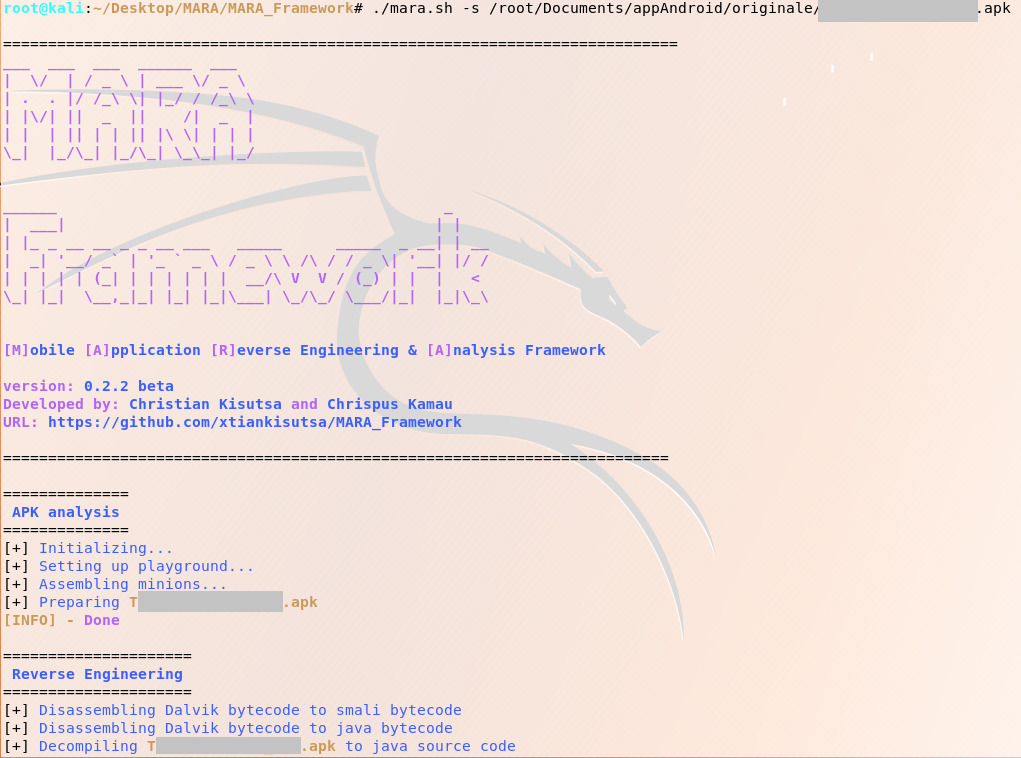
\includegraphics[width=.45\textwidth]{mara/MARAexecution01BN}\label{fig:maraScanA}} \quad
		\subfloat[]{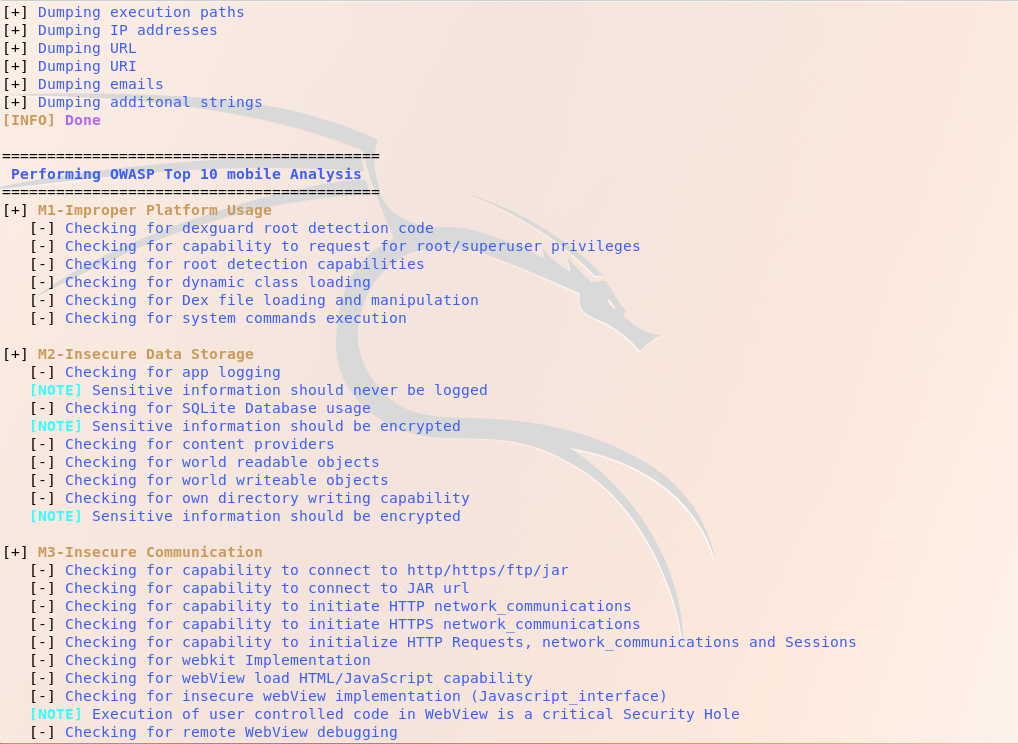
\includegraphics[width=.45\textwidth]{mara/MARAexecution03BN}\label{fig:maraScanB}}
	}
	\caption{Alcune delle operazioni effettuate da MARA.}
\end{figure}

Il primo passo effettuato è il reverse engineering dell'apk. Al suo interno, MARA ha a disposizione strumenti come \emph{apktool}, \emph{baksmali}, \emph{enjarify} e \emph{jadx}, in grado di ricavare il codice sorgente partendo dall'apk. Come si può vedere dalla figura \ref{fig:source}, è stato effettivamente ottenuto il codice sorgente dell'applicazione che può essere analizzato tramite strumenti automatici (lo stesso MARA lo fa) o manualmente.

\begin{figure}[h]
	\centering 
	\fbox{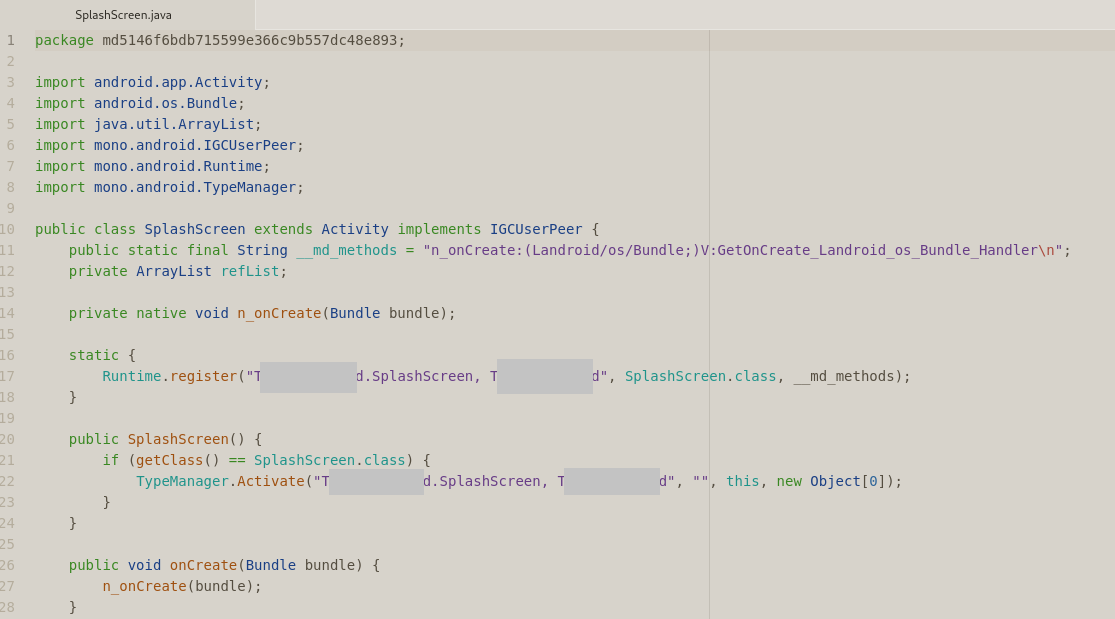
\includegraphics[width=.95\textwidth]{reverse/sourceBN2}} 
	\caption{Codice sorgente ottenuto.}
	\label{fig:source} 
\end{figure}

Successivamente si passa all'analisi del manifest, controllando activity, receiver e service eventualmente esportati. Vengono verificati i permessi ed altre opzioni ritenute pericolose o compromettenti (backup, debug, ecc.). Vengono estratti e controllati i certificati ed analizzato il codice sorgente alla ricerca di bug o comportamenti malevoli. Dopo queste verifiche preliminari, vengono eseguiti i controlli principali su cui si basa MARA; l'OWASP top 10 mobile (figura \ref{fig:maraScanB}). Come ultimo passo, vengono effettuati altri controlli standard come l'utilizzo di primitive crittografiche obsolete, utilizzo di connessioni non sicure, ecc.

%----------------------------------------------------%
%-------------------- SUPER -------------------------%
%----------------------------------------------------%

\section{SUPER Android Analyzer}

Il secondo strumento utilizzato è stato \ac{SUPER} Android Analyzer (figura \ref{fig:super}) \cite{SUPER}. 

\begin{figure}[h]
	\centering 
	
\includegraphics[width=.2\textwidth]{super/super} 
	\caption{SUPER logo.}
	\label{fig:super} 
\end{figure}

SUPER è un'applicazione a riga di comando, scritta in linguaggio Rust, che analizza file di tipo apk in cerca di vulnerabilità. È in grado di effettuare il reverse engineering dell'apk ed applicare una serie di regole per determinare l'effettiva presenza di vulnerabilità all'interno dell'applicazione. 

La particolarità di RUST è la sua estrema estensibilità. Tutte le regole sono infatti memorizzate in un file (\emph{rules.json}) ed è sempre possibile modificare quelle esistenti o crearne di nuove. Di seguito un esempio di regola:

\lstinputlisting[caption=Esempio di regola SUPER]{code/super.json}

Utilizzando questa regola, se viene trovata una porzione di codice che rispecchia il valore nel campo \emph{regex} e viene garantito il permesso specificato nel campo \emph{permissions} (in questo caso WRITE EXTERNAL STORAGE), allora viene rilevata una vulnerabilità con livello di criticità \emph{high} (campo \emph{criticality}) e viene fornita la descrizione presente nel campo \emph{description}.

\begin{figure}[h]
	\centering 
	\fbox{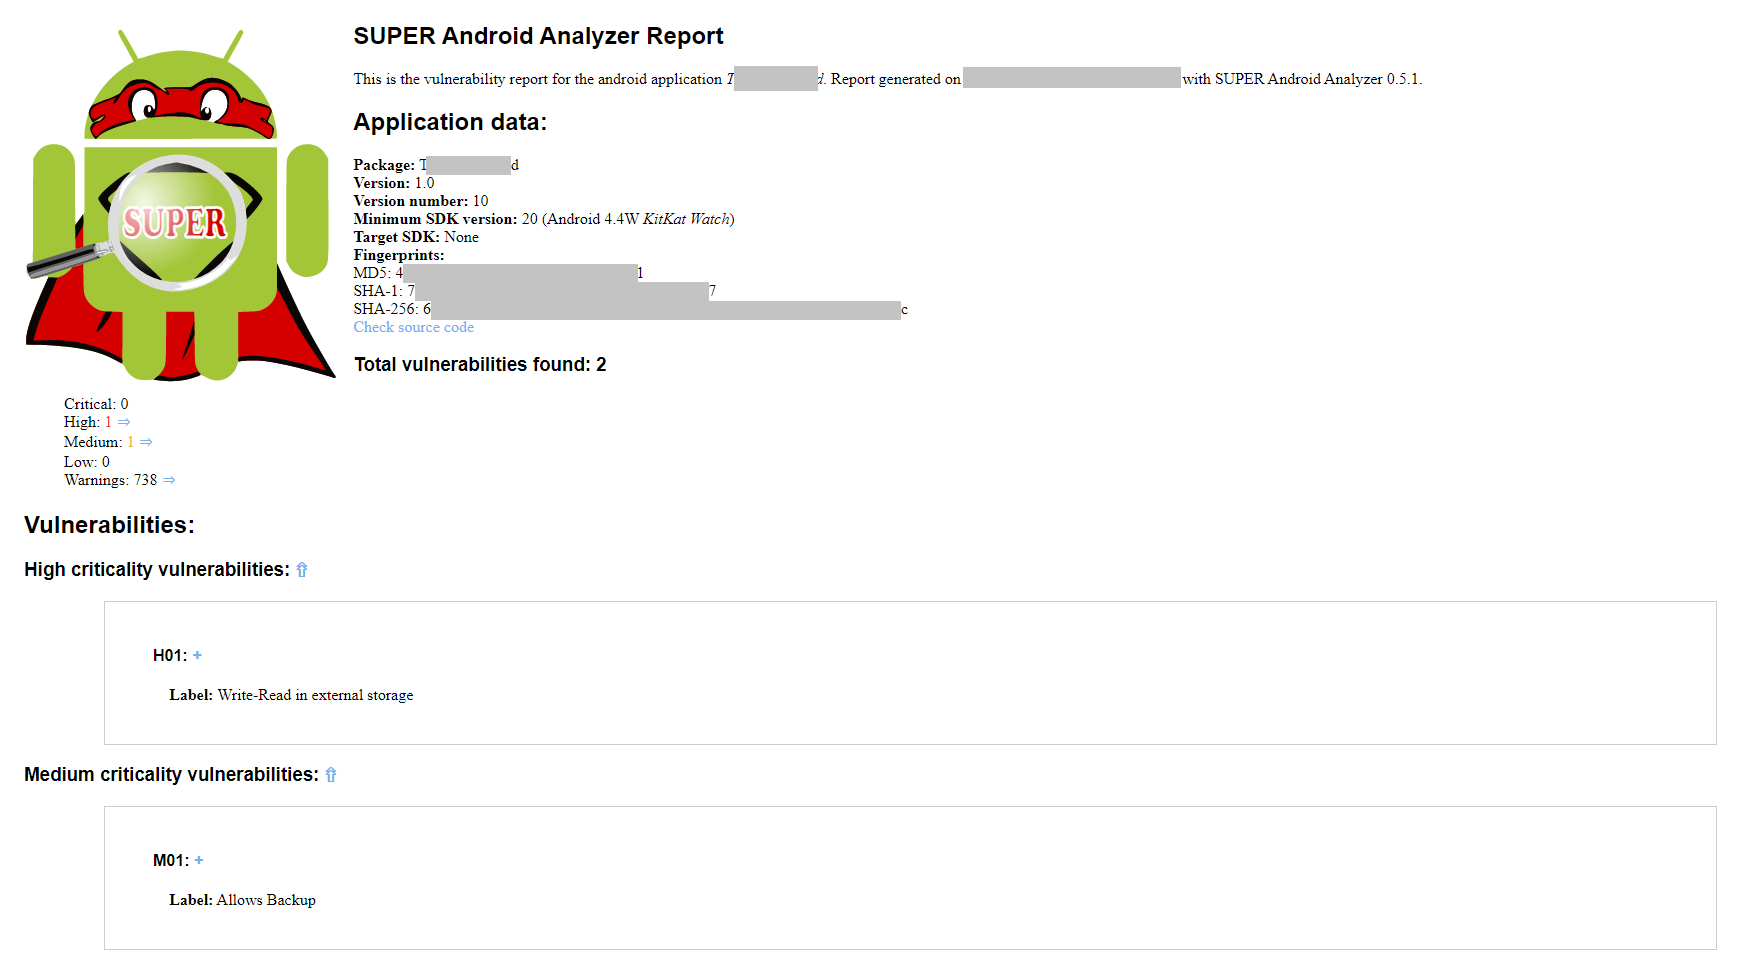
\includegraphics[width=.9\textwidth]{super/superResults}}
	\caption{Report di SUPER}
	\label{fig:superResults} 
\end{figure}

La scansione con SUPER genera un file html (figura \ref{fig:superResults}) nel quale, oltre a trovare informazioni di base sull'applicazione, è presente la lista delle vulnerabilità riscontrate che in questo caso sono una di livello alto ed una di livello medio. Espandendo la sezione relativa ad ogni vulnerabilità presente nel report, viene riportata la porzione di codice affetta dalla stessa (figura \ref{fig:superVuln}). 

\begin{figure}[h]
	\centering 
	\fbox{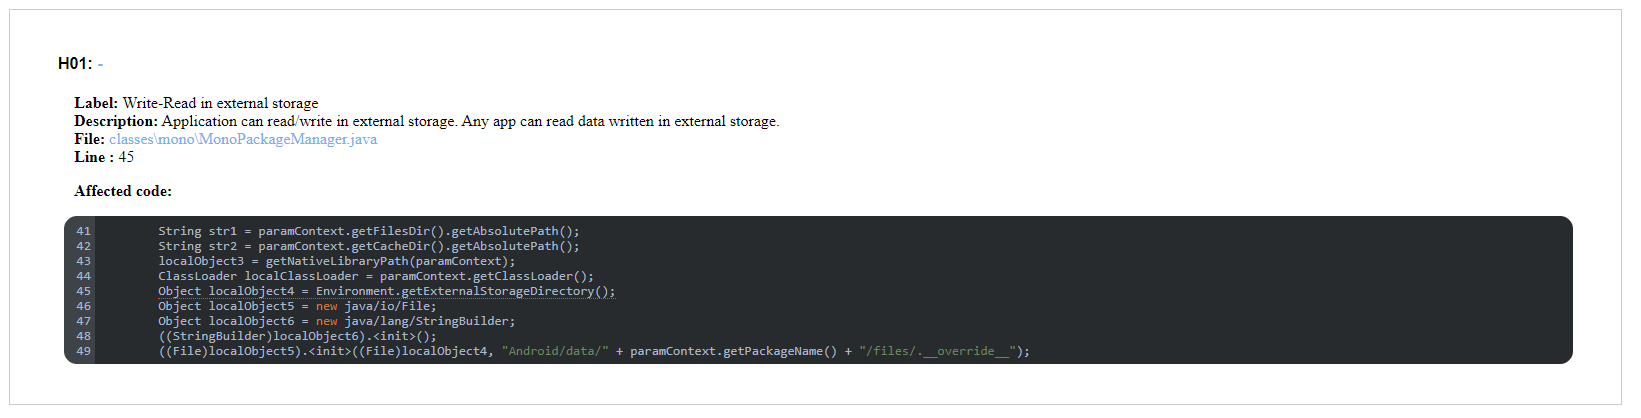
\includegraphics[width=.9\textwidth]{super/superVuln}} 
	\caption{Porzione di codice affetta dalla vulnerabilità}
	\label{fig:superVuln} 
\end{figure}

%----------------------------------------------------%
%--------------------- QARK -------------------------%
%----------------------------------------------------%

\section{QARK}
\begin{figure}[h]
	\centering 
	\fbox{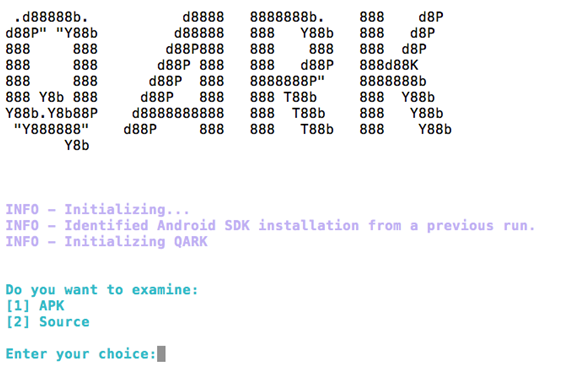
\includegraphics[width=.45\textwidth]{qark/QARK}}
	\caption{QARK}
	\label{fig:qark}
\end{figure}

L'ultimo strumento utilizzato è stato \ac{QARK} \cite{QARK} (figura \ref{fig:qark}). Le vulnerabilità sulle quali si concentra maggiormente sono le seguenti:
\begin{itemize}
	\item Componenti esportati inavvertitamente
	\item Intent vulnerabili ad intercettazioni
	\item Scorretta validazione dei certificati X.$509$
	\item Creazione di file world-readable o world-writeable
	\item Attività che possono far filtrare informazioni
	\item Utilizzo di Intent sticky
	\item Invio non sicuro di Broadcast Intent
	\item Informazioni hard-coded all'interno del codice
	\item Configurazioni potenzialmente vulnerabili delle WebView
	\item Tapjacking
	\item Applicazioni che abilitano il backup
	\item Applicazioni debuggabili
	\item Supporto ad API non aggiornate o con vulnerabilità note
\end{itemize}

La particolarità che contraddistingue QARK è la possibilità di generare comandi \ac{ADB} o interi apk in grado di sfruttare alcune delle vulnerabilità rilevate.

Il risultato dell'analisi di QARK, viene fornito tramite un file html (figura \ref{fig:qarkResults}) contenente l'elenco dei singoli problemi rilevati, la relativa descrizione e il file che li origina.
\begin{figure}[h]
	\centering 
	\fbox{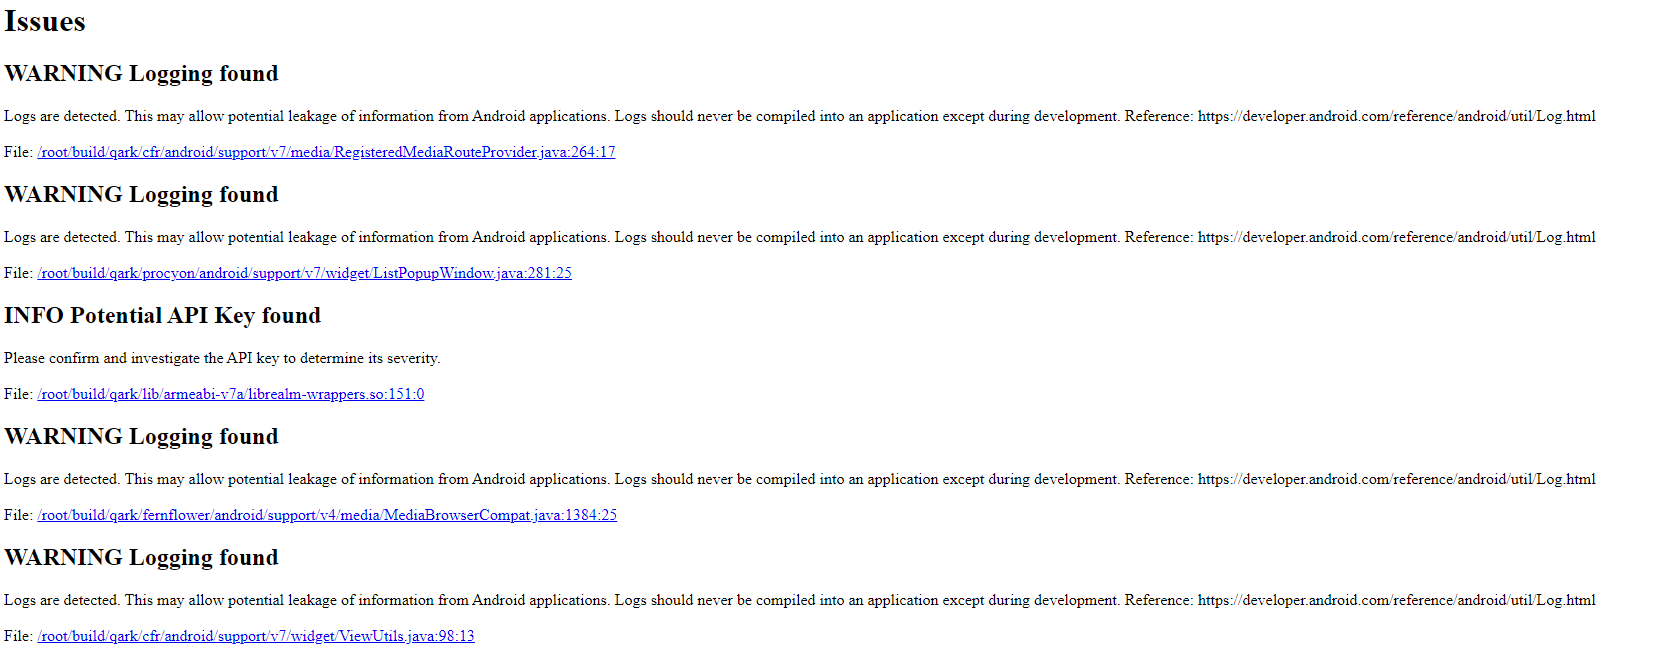
\includegraphics[width=.9\textwidth]{qark/QARKresults}}
	\caption{Risultati forniti dalla scansione di QARK.}
	\label{fig:qarkResults}
\end{figure}
\chapter{Analisi dinamiche}
In questa sezione verranno presentati gli strumenti utilizzati per effettuare le scansioni dinamiche. I risultati verranno aggregati e commentati insieme a quelli delle analisi statiche nella sezione $3$.

%----------------------------------------------------%
%-------------------- DROZER ------------------------%
%----------------------------------------------------%

\section{Drozer}

\begin{figure}[h]
	\centering 
	
\includegraphics[width=.45\textwidth]{/drozer/logo} 
	\caption{Drozer}
	\label{fig:drozer}
\end{figure}

Drozer\cite{Drozer} è un software open source, rilasciato e mantenuto da MWR InfoSecurity e licenziato tramite BSD. Drozer permette di assumere il ruolo di un'applicazione Android installata all'interno del dispositivo e di interagire con le altre applicazioni presenti.

Attraverso l'utilizzo di un agent Drozer si può fare tutto quello che un'applicazione installata nel dispositivo può fare (interagire con la Dalvik VM, utilizzare il meccanismo di \ac{IPC} o interagire col sistema operativo sottostante). L'agent fungerà da interfaccia di amministrazione remota e rappresenterà un'applicazione non privilegiata. L'agent richiede un solo permesso al sistema operativo: il permesso INTERNET, necessario per aprire la socket e connettersi con la console o il server. 

Drozer è in grado di costruire contenuti malevoli per eseguire exploit su vulnerabilità note e di caricarle sull'agent.

A seconda dei permessi concessi all'applicazione vulnerabile, Drozer è in grado di installare un agent completo, iniettare un agent limitato dentro al processo relativo all'applicazione o generare una reverse shell.

La particolarità di Drozer sta nell'assoluta indipendenza da strumenti come ADB o \ac{AAPT} che richiederebbero una connessione USB al dispositivo. Essa avviene infatti esclusivamente tramite rete (di default sulla porta TCP:$31415$).

\subsection{Utilizzo}
Drozer è in grado di eseguire avariate azioni:
\begin{itemize}
	\item \textbf{Ricavare le informazioni sui pacchetti installati nel dispositivo}. Questo comando dispone di numerosi filtri come ad esempio quello sui permessi richiesti. Nella figura \ref{fig:drozerList} sono state listate le applicazioni che richiedono il permesso RECORD AUDIO tra le quali compare anche l'applicazione che stiamo testando.
	\begin{figure}[h]
		\centering 
		\fbox{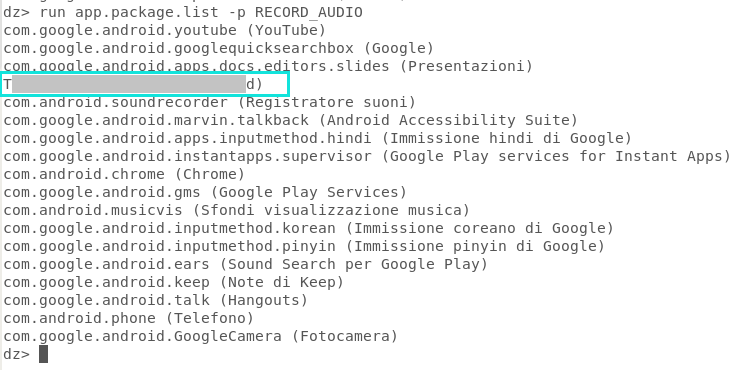
\includegraphics[width=.9\textwidth]{/drozer/drozerListBN}} 
		\caption{Elenco di applicazioni che richiedono il permesso RECORD AUDIO.}
		\label{fig:drozerList}
	\end{figure}

	\item \textbf{Ricavare le informazioni su un singolo pacchetto}. Il comando utilizzato nella figura \ref{fig:appInfo} permette di ricavare le informazioni di base di qualsiasi applicazione installata nel dispositivo. In questo caso sono le informazioni riguardanti l'applicazione testata.
	\begin{figure}[h]
		\centering 
		\fbox{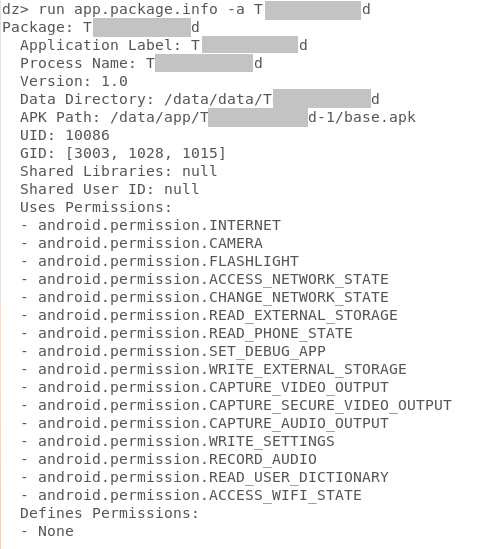
\includegraphics[width=.6\textwidth]{/drozer/appInfoBN}} 
		\caption{Informazioni sull'applicazione testata.}
		\label{fig:appInfo}
	\end{figure}

	\item \textbf{Identificare la possibile superficie d'attacco di un'applicazione}. Questo comando cerca componenti esportati (activities, broadcast receivers e content providers) o per i quali è attivata la modalità di \emph{debug}. Nell'applicazione sotto test, si può notare come l'unico componente esportato sia l'activity principale (figura \ref{fig:attackSurface}) e che la modalità di debug non sia attiva su alcun componente.
	\begin{figure}[h]
		\centering 
		\fbox{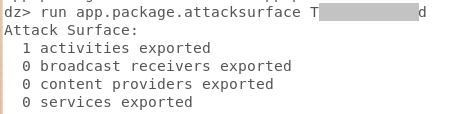
\includegraphics[width=.7\textwidth]{/drozer/attackSurfaceBN}} 
		\caption{Analisi della superficie d'attacco.}
		\label{fig:attackSurface}
	\end{figure}

	\item \textbf{Elencare e lanciare tutte le activities esportate da un'applicazione}. L'esecuzione dei due comandi riportati in figura \ref{fig:activities} rispettivamente, elencano tutte le activities esportate da un'applicazione e le eseguono. Nel nostro caso, l'unica activity esportata è quella che carica la schermata principale e la sua esecuzione fa semplicemente partire l'applicazione. 
	\begin{figure}[h]
		\centering 
		\fbox{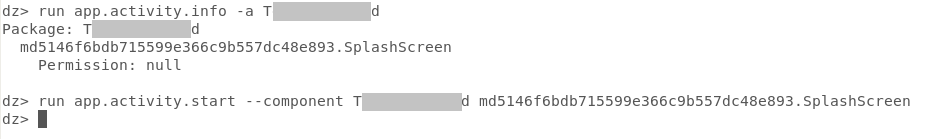
\includegraphics[width=.8\textwidth]{/drozer/activityBN}} 
		\caption{Elenco delle attività ed esecuzione.}
		\label{fig:activities}
	\end{figure}

	\item \textbf{Interagire con i \emph{content providers}}. È possibile listare ed interagire con i content providers esportati dalle applicazioni. Drozer fornisce anche uno scanner che mette insieme diverse tecniche per trovare paths ed inferire liste di possibili URI accessibili. È in grado anche di effettuare SQL injection se vengono rilevati database SQLite. Purtroppo nell'applicazione testata non sono presenti content providers e il risultato è vuoto (figura \ref{fig:provider}).
	\begin{figure}[h]
		\centering 
		\fbox{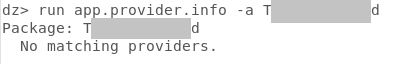
\includegraphics[width=.7\textwidth]{/drozer/providerBN}} 
		\caption{Elenco dei provider esportati.}
		\label{fig:provider}
	\end{figure}

	\item \textbf{Interagire con i servizi}. Come per i content providers, è possibile interagire con i servizi esportati. Anche in questo caso però, l'applicazione non presenta servizi esportati e quindi il risultato è vuoto (figura \ref{fig:services}).
	\begin{figure}[h]
		\centering 
		\fbox{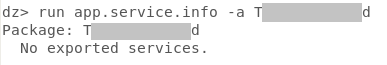
\includegraphics[width=.7\textwidth]{/drozer/servicesBN}} 
		\caption{Elenco dei servizi esportati.}
		\label{fig:services}
	\end{figure}

	\item \textbf{Opzioni avanzate}. Ulteriori comandi permettono di eseguire operazioni avanzate. \emph{shell.start} ad esempio, fa partire una shell linux interattiva sul dispositivo oppure \emph{tools.setup.busybox} vi installa \emph{busybox}.
\end{itemize}

%----------------------------------------------------%
%-------------------- SCROUNGER ---------------------%
%----------------------------------------------------%

\section{Scrounger}
\begin{figure}[h]
	\centering 
	
\includegraphics[width=.7\textwidth]{/scrounger/bannerBN} 
	\caption{Scrounger.}
	\label{fig:scrounger}
\end{figure}
Scrounger\cite{Scrounger} è uno strumento multipiattaforma (Android e IoS) dall'utilizzo simile a \emph{Metasploit}. Si presenta infatti con una console dalla quale è possibile eseguire dei comandi ed è composto da svariati moduli che permettono di automatizzare molte azioni necessarie nell'assessment di sicurezza di una applicazione mobile. È anche possibile scrivere i propri moduli ed eseguirli nella console principale del programma.

\subsection{Utilizzo}
Quando viene lanciato, Scrounger si presenta con una console molto simile a Metasploit dalla quale possiamo ad esempio elencare tutti i possibili moduli che riguardano Android (figura \ref{fig:lista}).
\begin{figure}[h]
	\centering 
	\fbox{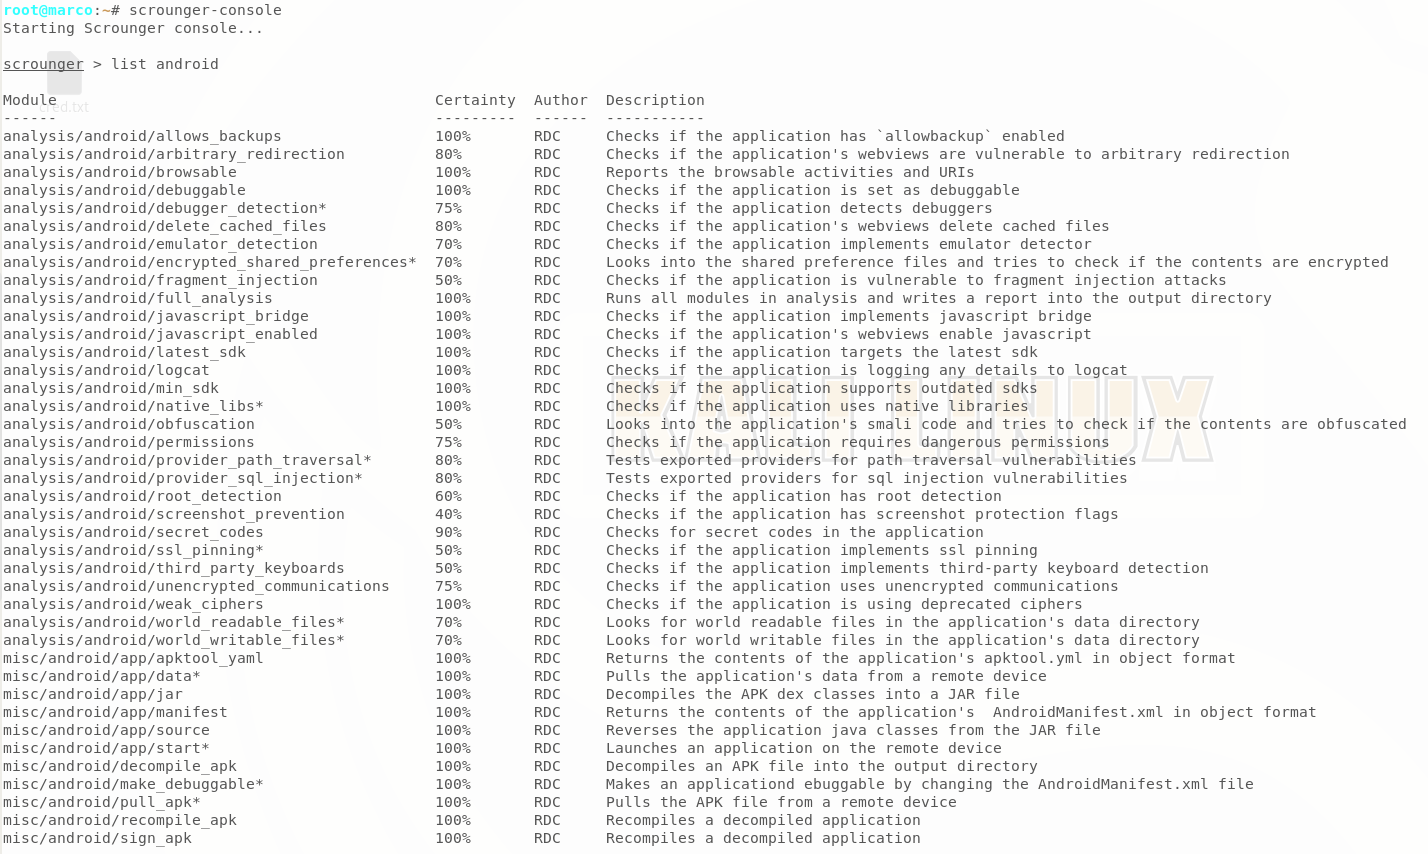
\includegraphics[width=.9\textwidth]{/scrounger/listaBN}}
	\caption{Moduli Android.}
	\label{fig:lista}
\end{figure}

Se volessimo verificare la possibilità di effettuare backup della nostra applicazione, potremmo utilizzare il modulo \emph{analysys/android/allow-backup} (figura \ref{fig:example}).
\begin{figure}[h]
	\centering 
	\fbox{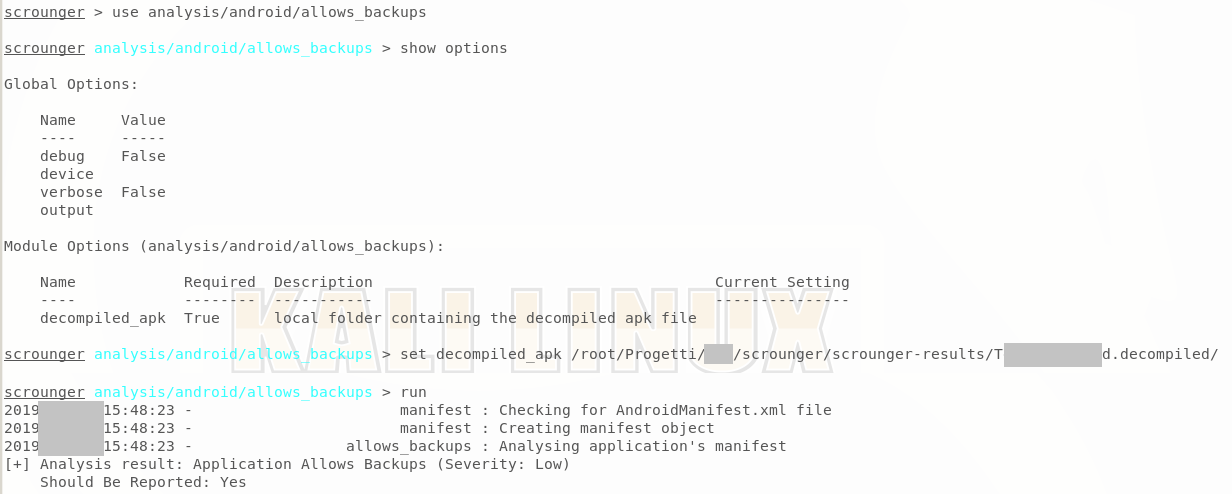
\includegraphics[width=.9\textwidth]{/scrounger/exampleCensBN}} 
	\caption{Un modulo di Scrounger.}
	\label{fig:example}
\end{figure}

Tramite il modulo \emph{android$/$full-analysys} è possibile eseguire automaticamente tutti i moduli inerenti ad Android. Per utilizzarlo è necessario collegare un device (meglio se con disponibilità dei privilegi di root) tramite adb che verrà utilizzato da Scrounger come ambiente di test nel quale installerà ed eseguirà l'applicazione da controllare.

È possibile utilizzare Scrounger anche direttamente da linea di comando (figura \ref{fig:start}) ed è infatti in questa modalità che è stata eseguita l'analisi dell'applicazione (l'opzione \emph{-f} indica proprio il modulo \emph{full-analysys}).
\begin{figure}[h]
	\centering 
	\fbox{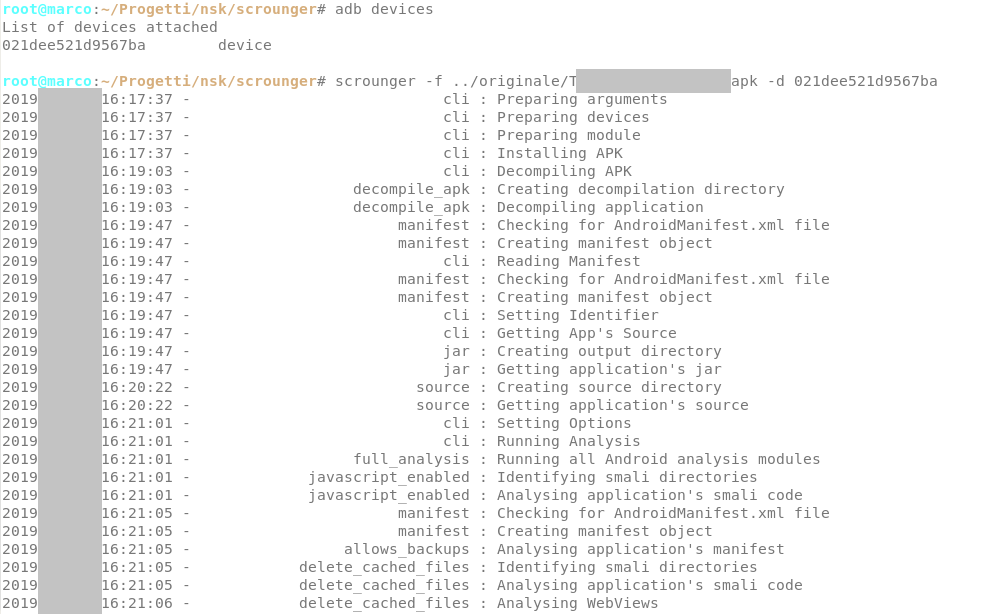
\includegraphics[width=.9\textwidth]{/scrounger/startCensBN}} 
	\caption{Full analysys.}
	\label{fig:start}
\end{figure}

Una volta terminata la scansione, i risultati vengono visualizzati a schermo e viene generato un report in formato \emph{JSON}.
\chapter{Risultati}

In questa sezione verranno presentati i risultati ottenuti dalle varie scansioni.
\begin{table}[h]
	{\footnotesize
	\begin{center}
		\begin{tabular}{|c||c|c|c|c|c|}
			\hline 
			\textbf{Vulnerabilità} 	& \textbf{MARA} & \textbf{SUPER}& \textbf{QARK} & \textbf{Drozer}	& \textbf{Scrounger}	\\ 
			\hline \hline
			Codice non offuscato 	& \Checkmark	&  				&  				& \Checkmark 		&  						\\ 
			\hline 
			Possibile backup 		& \Checkmark 	& \Checkmark 	& \Checkmark 	&  					& \Checkmark			\\ 
			\hline 
			Attività di Logging 	& \Checkmark 	&  				& \Checkmark 	&  					& \Checkmark 			\\ 
			\hline 
			Uso librerie esterne 	& \Checkmark 	&  				&  				&  					& \Checkmark 			\\ 
			\hline 
			R$/$W memoria esterna 	&  				& \Checkmark 	& \Checkmark 	&  					& \Checkmark 			\\ 
			\hline 
			No pinning SSL 			&  				&  				&  				&  					& \Checkmark 			\\ 
			\hline 
			Webviews vulnerabili 	&  				& 				&  				&  					& \Checkmark 			\\ 
			\hline 
			Connessioni non sicure 	& \Checkmark	& \Checkmark 	& \Checkmark 	&  					&  						\\ 
			\hline 
			Possibili screenshot 	&  				&  				&  				&  					& \Checkmark 			\\ 
			\hline 
			Non rileva debuggers 	&  				&  				&  				&  					& \Checkmark 			\\ 
			\hline 
			Activity esportata 		& \Checkmark 	&  				& \Checkmark 	& \Checkmark 		&  						\\ 
			\hline 
			Non rileva emulatori 	&  				&  				&  				&  					& \Checkmark  			\\ 
			\hline 
			Permessi pericolosi 	& \Checkmark 	& \Checkmark 	&  				&  					& \Checkmark 			\\ 
			\hline 
			Non controlla root 		&  				&  				&  				&  					& \Checkmark 			\\ 
			\hline 
		\end{tabular}
	\end{center}
	}
	\caption{Sommario risultati.}
	\label{tab:results} 
\end{table}

Nella tabella \ref{tab:results} sono state raccolte le principali vulnerabilità rilevate indicando per ognuna il tool responsabile della sua individuazione. Passiamo adesso ad un'analisi più approfondita dei risultati.

\section{Codice non offuscato}

\begin{figure}[h]
	\centering 
	\fbox{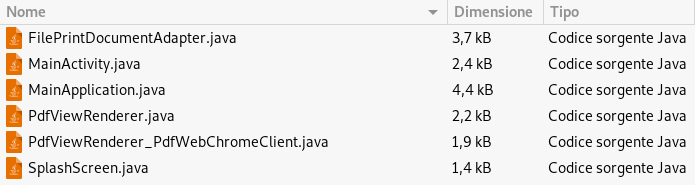
\includegraphics[width=.9\textwidth]{reverse/sources}}
	\caption{File JAVA ottenuti dall'apk.}
	\label{fig:sources}
\end{figure}

\subsection{Descrizione della vulnerabilità}

Un'applicazione Android viene definita vulnerabile al \emph{reverse engineering} quando un attaccante può essere in grado di effettuare una delle seguenti operazioni\cite{reverse}:
\begin{itemize}
	\item Risalire al codice sorgente originale partendo dai file binari
	\item Ottenere il contenuto di una \emph{string table} binaria
	\item Eseguire analisi \emph{cross functional}
\end{itemize}

L'offuscamento del codice è quel processo tramite il quale viene modificato l'eseguibile in maniera tale da non essere più facilmente interpretabile dall'attaccante mantenendo le stesse funzionalità dell'originale.

Partendo dal presupposto che con adeguati sforzi ed abbastanza tempo si può rivelare il codice sorgente di pressoché qualunque applicazione Android tramite  reverse engineering, su quella testata non è stato applicato alcun processo di offuscamento. Tale mancanza ha permesso la decompilazione dell'apk originale quasi ad ogni strumento a mia disposizione (figura \ref{fig:source} e \ref{fig:sources}).

Le possibili varianti di offuscamento sono tantissime e svariano dalla ridenominazione di variabili o funzioni (figura \ref{fig:reverse1}), alla crittazione delle stringhe (figura \ref{fig:reverse2}), all'inserimento di codice inutilizzato o alla modifica del flusso di esecuzione.

\begin{figure}[h]
	\centering
	\subfloat[]{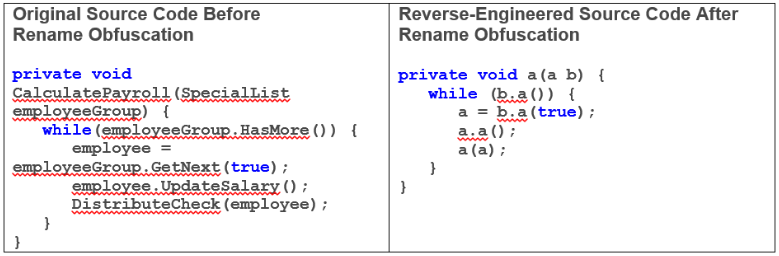
\includegraphics[width=.9\textwidth]{reverse/reverse1}\label{fig:reverse1}} \\
	\subfloat[]{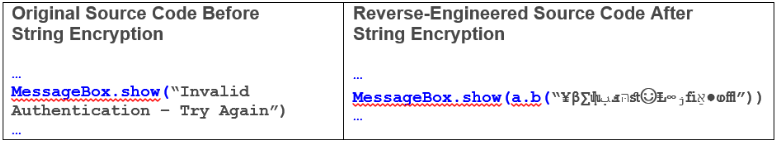
\includegraphics[width=.9\textwidth]{reverse/reverse2}\label{fig:reverse2}}
	\caption{Esempi di offuscamento del codice.}
	\label{fig:obfuscation}
\end{figure}

\subsection{Contromisure}
È consigliabile utilizzare una o più tecniche di offuscamento del codice. È importante notare che l'utilizzo di alcune di queste tecniche può comportare un calo delle prestazioni a causa delle operazioni di decodifica.

Esistono strumenti specifici in grado di applicare automaticamente le tecniche principali lasciando all'utente l'unico compito di trovare il giusto compromesso tra offuscamento e prestazioni.

\section{Possibile backup}

\begin{figure}[h]
	\centering 
	\fbox{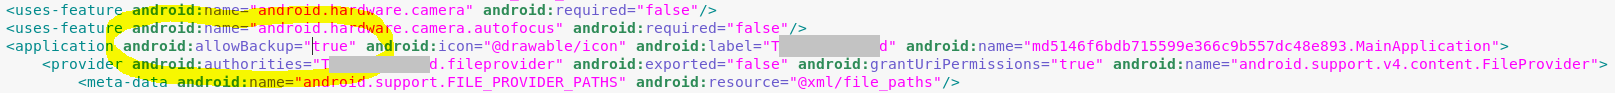
\includegraphics[width=.9\textwidth]{backup/backup}}
	\caption{Estratto dal manifest.}
	\label{fig:backup}
\end{figure}

\subsection{Descrizione della vulnerabilità}

Come visibile in figura \ref{fig:backup}, è presente nel manifest l'opzione:
\begin{center}
	\emph{android:allowBackup="true"}
\end{center}

Con questa opzione attiva è possibile effettuare un backup completo dell'applicazione che, con i privilegi di root, può comprendere anche le \emph{shared preference}, tutti i file, i database e l'apk stesso.
\begin{figure}[h]
	\centering 
	\fbox{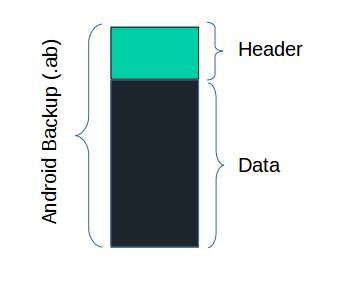
\includegraphics[width=.5\textwidth]{backup/exploit}}
	\caption{Formato backup app Android.}
	\label{fig:structure}
\end{figure}

Analizzando poi la struttura di un backup Android (figura \ref{fig:structure}) e sapendo che nell'intestazione non è presente alcun riferimento ai dati contenuti nel backup, diventa chiara l'esposizione ad un attacco che permette di modificare i dati contenuti nel backup e reinserire la nuova versione modificata nel dispositivo. Tale attacco può essere riassunto in questi passaggi:

\begin{itemize}
	\item Ottenere il backup (tramite adb ad esempio)
	\item Separare i dati dall'intestazione del backup
	\item Modificare a piacimento i dati dell'applicazione
	\item Reimpacchettare i nuovi dati
	\item Recuperare l'intestazione dal backup originale
	\item Anteporre l'intestazione ai nuovi dati
	\item Ripristinare il backup  con i nuovi dati nel dispositivo (esso verrà accettato senza alcuna richiesta dato che verrà riconosciuto l'intestazione dell'applicazione originale)
\end{itemize}

\subsection{Contromisure}

Evitare questo tipo di attacco è molto semplice; se non è strettamente necessario dover effettuare backup dell'applicazione, è sufficiente settare l'opzione \emph{android:allowBackup} a false e sarà il sistema operativo stesso a non permettere tale operazione.

\section{Attività di logging}

\begin{figure}[h]
	\centering 
	\fbox{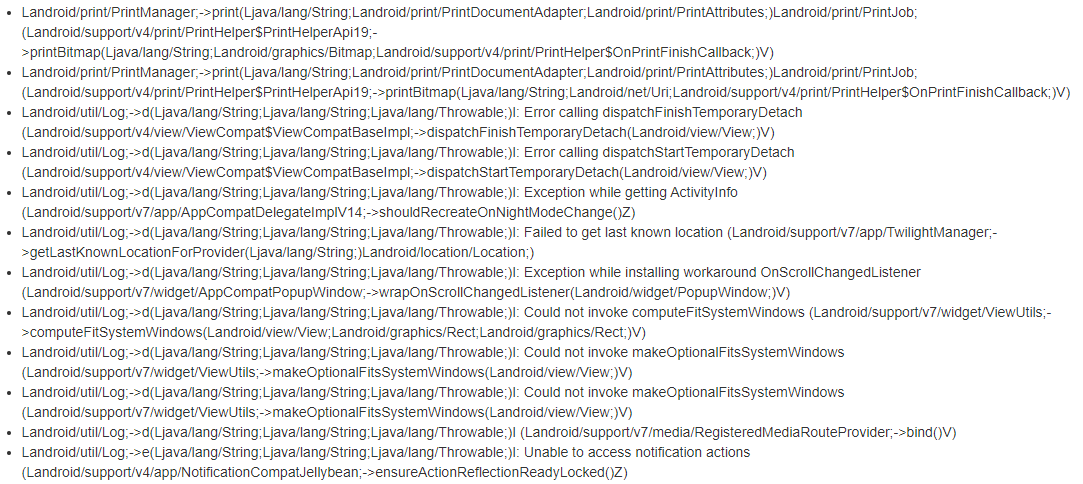
\includegraphics[width=.9\textwidth]{log}}
	\caption{Alcune funzioni che loggano informazioni.}
	\label{fig:log}
\end{figure}

\subsection{Descrizione della vulnerabilità}

Nell'applicazione sono presenti $454$ chiamate a funzioni di log (figura \ref{fig:log}). Alcune di queste potrebbero svelare informazioni riservate o utili all'attaccante.

Analizzando i log non sembra essere presente un rilascio di informazioni utili ma, data la quantità delle funzioni di log presenti, non è stato possibile controllarle tutte approfonditamente. Un attaccante con abbastanza tempo a disposizione potrebbe analizzare completamente i log generati ed ottenere informazioni interessanti.

\subsection{Contromisure}
In questo caso, la pratica migliore è quella di cercare di loggare il minor numero di informazioni possibile; è quindi consigliabile controllare l'effettiva necessità di tutte le funzioni di log presenti rimuovendo eventualmente quelle non necessarie.

\section{Uso di librerie esterne}

\begin{figure}[h]
	\centering 
	\fbox{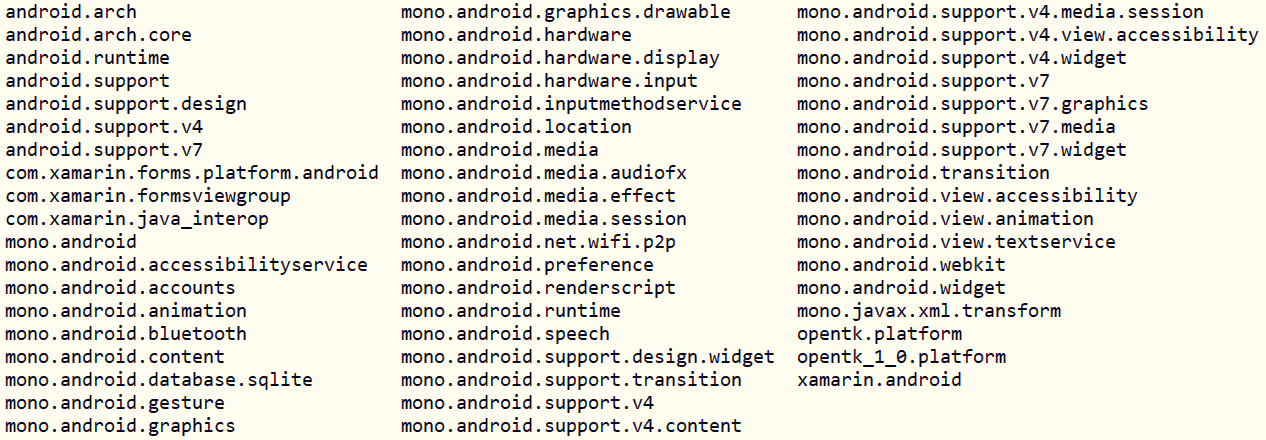
\includegraphics[width=.9\textwidth]{librerie}}
	\caption{Librerie esterne utilizzate.}
	\label{fig:librerie}
\end{figure}

\subsection{Descrizione della vulnerabilità}

All'interno dell'applicazione sono state rilevate un gran numero di librerie esterne (figura \ref{fig:librerie}). Molti strumenti automatici importano automaticamente librerie che possono anche non essere mai utilizzate dallo sviluppatore. Al contrario, l'utilizzo di alcune librerie accelera il processo di sviluppo ma può portare a due tipi di effetti indesiderati:

\begin{itemize}
	\item Una libreria può contenere una vulnerabilità che può rendere vulnerabile l'intera applicazione.
	\item Una libreria può utilizzare una licenza (ad esempio la LGPL$3$) che richiede al creatore dell'applicazione di fornire agli utilizzatori l'accesso al codice sorgente dell'intera applicazione che ne fa uso.
\end{itemize}

\subsection{Contromisure}
Per i motivi esposti sopra, occorre sempre utilizzare il minor numero possibile di librerie esterne, controllando per ognuna la licenza e la presenza di vulnerabilità note.

\section{Permessi pericolosi}

\begin{figure}[h]
	\centering 
	\fbox{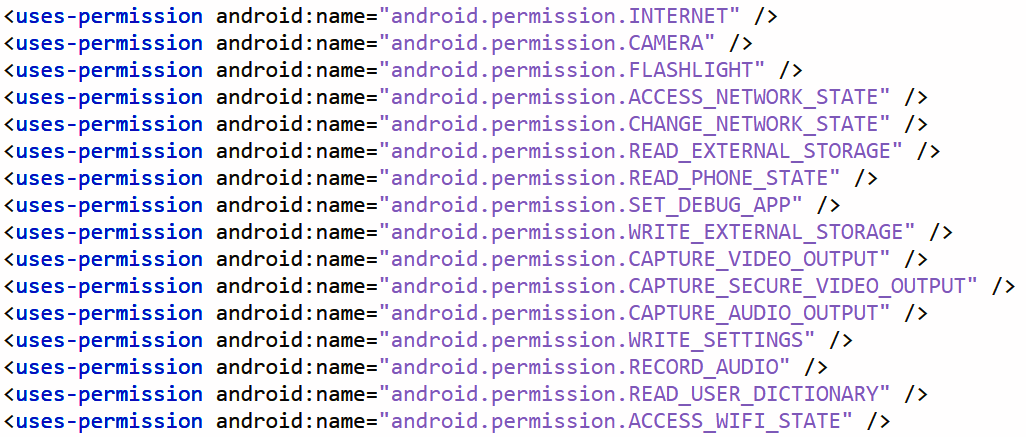
\includegraphics[width=.9\textwidth]{permessi}}
	\caption{Permessi richiesti dall'applicazione.}
	\label{fig:permessi}
\end{figure}

\subsection{Descrizione della vulnerabilità}

Estraendo dal manifest i permessi richiesti dall'applicazione (figura \ref{fig:permessi}) se ne notano alcuni il cui utilizzo può risultare molto pericoloso. 

L'accoppiata \emph{READ EXTERNAL STORAGE} e \emph{WRITE EXTERNAL STORAGE} in particolare, permette all'applicazione l'accesso (in lettura e scrittura) alla memoria esterna del dispositivo. Tale memoria non è protetta dal sistema di isolamento di Android e qualunque file lì presente può essere letto$/$scritto da qualunque applicazione possegga il relativo permesso. Se un attaccante riuscisse a prendere possesso dell'applicazione, potrebbe dunque leggere e scrivere qualunque file, di qualunque applicazione, presente nella memoria esterna.

Da un'analisi dell'applicazione è stato rilevato anche che in realtà la memoria esterna non viene mai utilizzata e quindi la dichiarazione di tali permessi è completamente inutile se non pericolosa.

\subsection{Contromisure}
Come precedentemente detto, è fondamentale richiedere il minor numero di permessi possibili, solo quelli strettamente necessari al funzionamento dell'applicazione. Aggiungere permessi inutilizzati ha come unico risultato l'esposizione ad attacchi o utilizzi non previsti (anche illeciti) della stessa.

In questo caso occorre controllare l'effettivo utilizzo e la necessità di ogni singolo permesso richiesto, rimuovendo eventualmente quelli inutilizzati.

\section{Mancata implementazione pinning SSL}

\subsection{Descrizione della vulnerabilità}
Il \emph{pinning} di un certificato è l'associazione del server di backend con uno specifico certificato X.$509$ o una chiave pubblica. Una volta inserito tale certificato/chiave nell'applicazione tramite \emph{hardcoding} o alla prima connessione, si può essere ragionevolmente sicuri che l'applicazione si connetta solamente al server conosciuto evitando possibili attacchi \ac{MITM}.

Il pinning del certificato alla prima connessione dell'applicazione con il server non fornisce comunque una protezione completa se effettuata in un ambiente non controllato. L'attaccante potrebbe comunque intercettare la prima connessione, fornire il proprio certificato che a questo punto verrebbe riconosciuto come legittimo. 

L'implementazione più sicura del pinning dei certificati sarebbe quella dell'hardcoding all'interno dell'applicazione ma questa soluzione crea problemi nel caso di modifiche successive del certificato (scadenza, revoca, ecc...). Per questo motivo, al posto del certificato, si tende ad effettuare il pinning della chiave pubblica del server che dovrebbe avere una durata più estesa.

\subsection{Contromisure}

\begin{figure}[h]
	\centering 
	\fbox{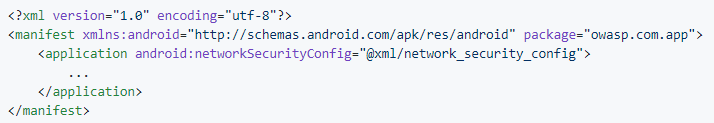
\includegraphics[width=.9\textwidth]{pinning/manifest}}
	\caption{Modifica al manifest.}
	\label{fig:pinningManifest}
\end{figure}

Dall'analisi del codice sorgente dell'applicazione è emersa l'assenza di questo sistema di protezione. Android (dalla versione $7.0$ in poi) fornisce il \emph{Network Security Configuration}, un sistema che permette di impostare una connessione sicura senza modificare il codice sorgente. Le uniche modifiche da effettuare (dopo aver ottenuto un certificato) sono: 
	\begin{itemize}
		\item Aggiungere al manifest la dichiarazione di un file di configurazione di \emph{network security}(figura \ref{fig:pinningManifest}).
		\item La creazione di un file di configurazione (figura \ref{fig:pinningFile}) nel quale inserire un pool di chiavi ritenute affidabili per connettersi al server.
	\end{itemize}

\begin{figure}[h]
	\centering 
	\fbox{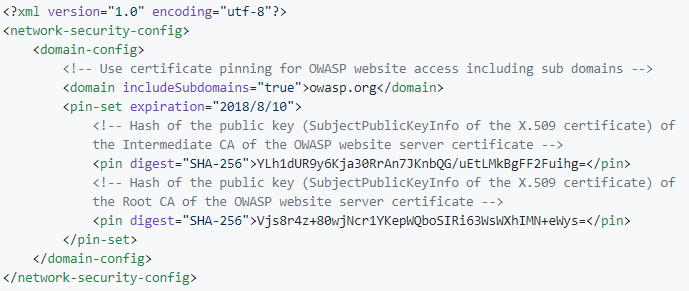
\includegraphics[width=.9\textwidth]{pinning/file}}
	\caption{Modifica al manifest.}
	\label{fig:pinningFile}
\end{figure}

\section{Connessioni non sicure}

\subsection{Descrizione della vulnerabilità}
Le analisi statiche dell'applicazione hanno rilevato $540$ possibili connessioni \ac{HTTP}. Le connessioni \ac{HTTP} sono intrinsecamente insicure in quanto non cifrate in alcun modo. Il traffico in chiaro può quindi essere intercettato e compreso dall'attaccante senza particolari sforzi.

L'analisi manuale del codice ha trasformato questa rilevazione in un falso positivo dato che gli \ac{URL} rilevati sono semplicemente gli schemi dei vari file \ac{XML} (figura \ref{fig:schema}).

\begin{figure}[h]
	\centering 
	\fbox{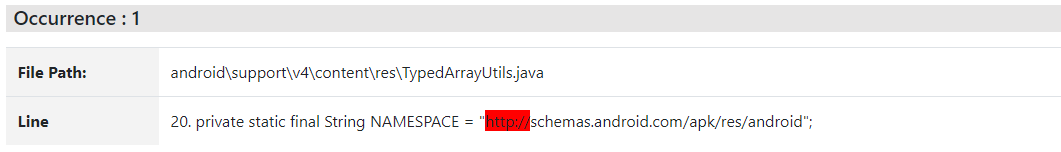
\includegraphics[width=.9\textwidth]{http}}
	\caption{XML schema.}
	\label{fig:schema}
\end{figure}

\subsection{Contromisure}
In generale, occorre sempre utilizzare connessioni \ac{HTTPS} al posto delle connessioni \ac{HTTP}, ma in questo caso non c'è bisogno di alcuna contromisura in quanto non si tratta di vere connessioni.

\section{Possibile screenshot}

\begin{figure}[h]
	\centering 
	\fbox{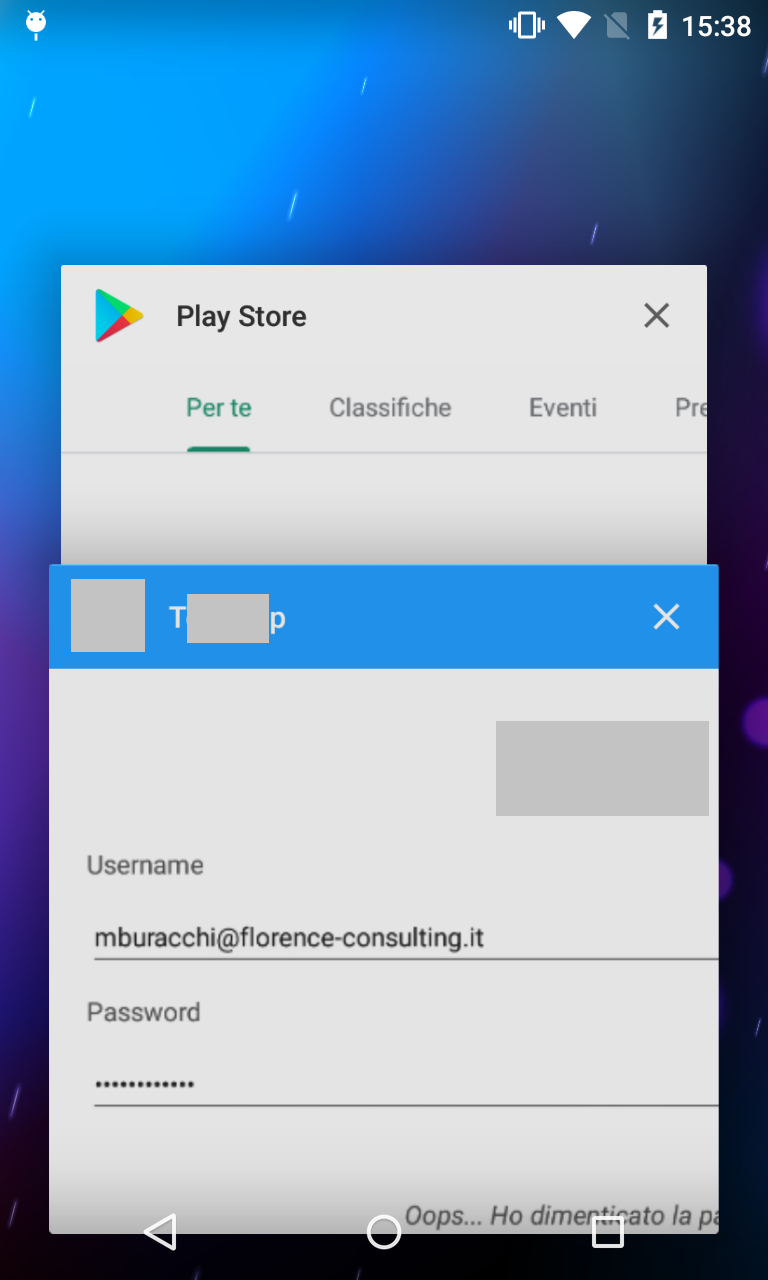
\includegraphics[width=.45\textwidth]{screen/background}}
	\caption{Background screenshot.}
	\label{fig:background}
\end{figure}

\subsection{Descrizione della vulnerabilità}
L'applicazione permette il salvataggio di screenshot. Tale pratica è spesso sconsigliata per due motivi:
\begin{itemize}
	\item Un'applicazione malevola potrebbe effettuare screenshot quando sono presenti dati sensibili sullo schermo (elenco clienti, utenti o transazioni) per ottenere informazioni altrimenti inaccessibili. Gli screenshot sono salvati nella memoria pubblica e possono essere recuperati da qualunque altra applicazione presente sul dispositivo.
	\item Ogni volta che l'applicazione viene messa in background, il sistema operativo effettua uno screenshot per riproporre l'ultima schermata al ritorno in foreground. Tale screenshot è visibile anche nell'elenco delle applicazioni in background (figura \ref{fig:background}).
\end{itemize}

\subsection{Contromisure}
È consigliabile bloccare la possibilità di effettuare screenshot dell'applicazione se non strettamente necessario. Per raggiungere questo obiettivo è sufficiente utilizzare l'opzione \emph{FLAG SECURE} nel metodo \emph{onCreate()} dell'activity che si vuole proteggere (figura \ref{fig:screen}).

\begin{figure}[h]
	\centering 
	\fbox{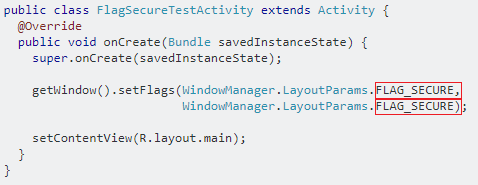
\includegraphics[width=.9\textwidth]{screen/flag}}
	\caption{Esempio di blocco degli screen.}
	\label{fig:screen}
\end{figure}

\section{Activity esportata}

\subsection{Descrizione della vulnerabilità}
L'applicazione esporta una activity. L'esportazione di una activity permette la sua invocazione da parte di un'altra applicazione o del sistema. Esportazioni non necessarie incrementano la superficie d'attacco a disposizione dell'attaccante. Fortunatamente l'unica activity esportata è quella necessaria per l'esecuzione dell'applicazione e quindi non rappresenta un problema da questo punto di vista. 

\subsection{Contromisure}
Nessuna contromisura necessaria.

\section{Non rileva emulatori$/$debuggers$/$root}

\subsection{Descrizione della vulnerabilità}
Al momento dell'installazione non viene controllato se l'ambiente in cui si eseguirà l'applicazione è sicuro. Eseguire in modalità particolari (ambienti di emulazione, ambienti di debug o dispositivi con permessi di root) un'applicazione che possiede informazioni sensibili, è sempre non sicuro. È quindi buona pratica effettuare dei controlli in merito. 

Nel caso ci trovassimo in un ambiente anomalo, non dovremmo permettere l'installazione dell'applicazione o quantomeno avvertire l'utente del rischio che si corre. 

\subsection{Contromisure}
Purtroppo non esiste una singola procedura per effettuare queste verifiche ma occorre implementare controlli multipli. Tra i più comuni troviamo i seguenti:
\begin{itemize}
	\item Controllare la presenza di alcuni file o binari abitualmente presenti in ambienti con privilegi di root sbloccati (superuser.apk, daemonsu, su, ecc...).
	\item Controllare la presenza del comando \emph{su} nel \emph{PATH}.
	\item Controllare a runtime la presenza di processi attivi riconducibili ad ambienti non sicuri.
	\item Tramite il gestore pacchetti di Android, verificare la presenza di applicazioni che operano in ambienti non sicuri.
	\item Controllare la modalità di montaggio delle partizioni del sistema. Quando si sbloccano i privilegi di root, esse vengono montate in modalità lettura$/$scrittura mentre normalmente sono montate in sola lettura.
	\item Controllare di non essere su una ROM custom. 
\end{itemize} 
\chapter{Applicazione contraffatta}

\section{Introduzione}

In questa sezione verrà illustrato un possibile attacco, eseguito sull'applicazione testata, che permette di ottenere il controllo totale sul dispositivo vittima. Verrà infatti creata una versione dell'applicazione indistinguibile dall'originale, ma contenente un trojan che instaurerà una connessione remota con l'attaccante permettendogli così l'accesso al dispositivo. Di seguito, il procedimento per effettuare questo tipo di attacco.

\section{Esecuzione}

\begin{figure}[h]
	\centering
	\fbox{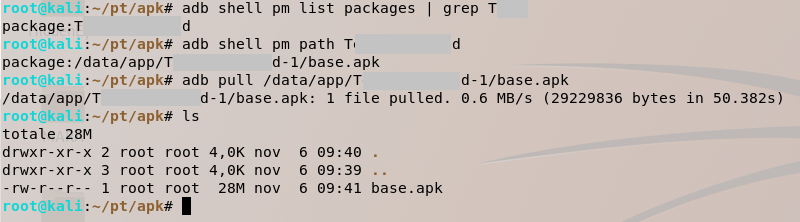
\includegraphics[width=.9\textwidth]{app/apk}}
	\caption{Ottenimento apk.}
	\label{fig:apk}
\end{figure}

L'unica cosa di cui si ha bisogno è l'apk originale. Esso può essere ottenuto in svariati modi. In questo caso è stato preso direttamente dal dispositivo della vittima tramite adb (figura \ref{fig:apk}).

Una volta ottenuto l'apk, utilizziamo \emph{msfvenom}\cite{MSFVenom} per iniettare la backdoor. Il comando viene lanciato indicando come payload da iniettare una connessione \emph{meterpreter}$/$\emph{reverse-tcp} chiedendo di instaurare la connessione all'IP $10.10.50.50$ (l'indirizzo remoto del computer dell'attaccante).

Come si può vedere nella figura \ref{fig:backdoor}, \emph{msfvenom} riconosce automaticamente la piattaforma (Android) e l'architettura (Dalvik) ed esegue i seguenti passi:

\begin{itemize}
	\item Crea una \emph{signing key} ed un \emph{keystore} che verranno utilizzati per firmare la nuova applicazione modificata.
	\item Decompila l'apk originale.
	\item Decompila l'apk del payload.
	\item Analizza il codice sorgente e localizza il punto nel quale iniettare il malware.
	\item Inietta il malware collegandolo alla activity principale.
	\item Aggiunge i permessi necessari a prendere il controllo del dispositivo.
	\item Effettua la build del nuovo apk.
	\item Allinea e firma il nuovo apk utilizzando le chiavi create in precedenza.
\end{itemize}

\begin{figure}[h]
	\centering
	\fbox{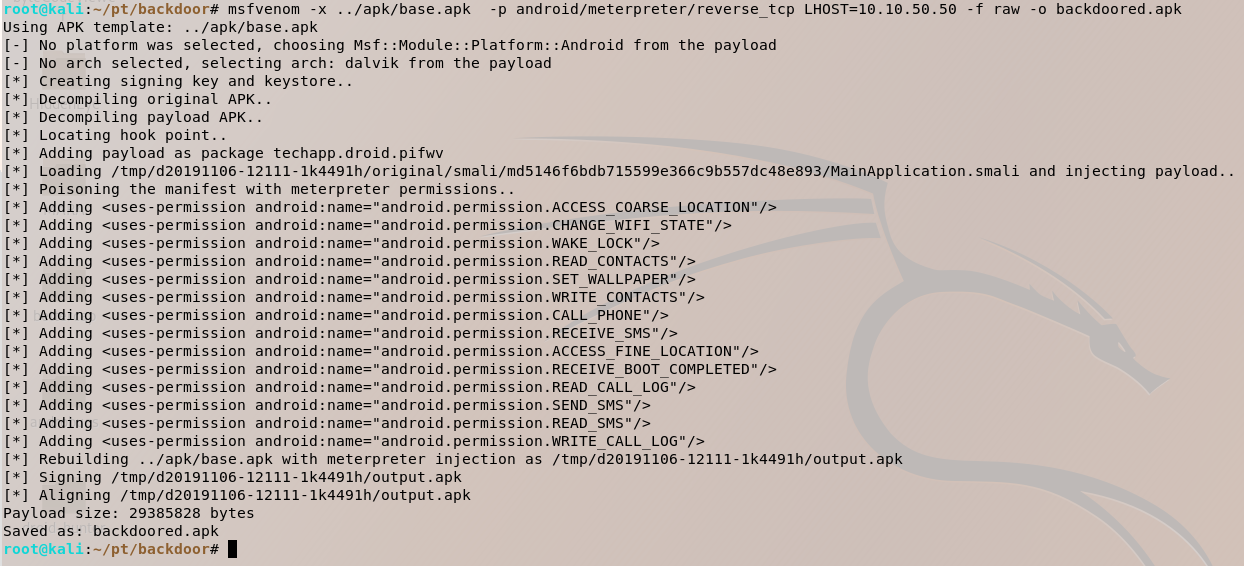
\includegraphics[width=.9\textwidth]{app/backdoor}} 
	\caption{Creazione backdoor.}
	\label{fig:backdoor} 
\end{figure}

Dopo aver creato l'applicazione malevola, l'attaccante lancia un server \ac{CC} tramite la piattaforma \emph{metasploit} (figura \ref{fig:metasploit}) e si mette in attesa di ricevere connessioni sulla porta $4444$. È possibile configurare l'exploit in modo che accetti connessioni dirette alla porta $4444$ da uno specifico IP (se conosciamo esattamente l'IP della vittima) o da qualunque IP (questa funzione si rivela molto utile in caso di IP dinamici).

\begin{figure}[h]
	\centering
	\fbox{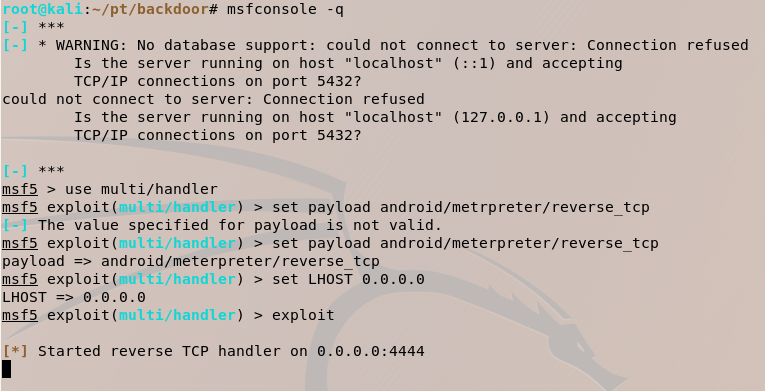
\includegraphics[width=.9\textwidth]{app/metasploit}} 
	\caption{Server C\&C.}
	\label{fig:metasploit} 
\end{figure}

Fino a questo punto non c'è stato bisogno di interagire con la vittima ed è stata creata tutta la struttura dell'attacco in maniera quasi automatica. L'intero processo non ha richiesto alcuna informazione oltre all'apk originale.

Adesso bisogna sfruttare la componente notoriamente più debole nell'ambito della cybersecurity: l'utente.

L'attaccante deve infatti convincere la vittima a scaricare ed installare l'applicazione contraffatta (supponendo che non abbia direttamente a disposizione il dispositivo, nel qual caso può provvedere direttamente all'installazione).

Il metodo migliore per ottenere questa collaborazione è sicuramente tramite operazioni di social-engineering. L'attaccante può ad esempio mandare una email alla vittima nella quale si richiede di aggiornare con la massima urgenza l'applicazione a causa di problemi di sicurezza. L'apk malevolo potrebbe essere spedito come allegato della mail insieme alle istruzioni su come installarlo. Un altro metodo potrebbe essere quello di fornire un link dal quale scaricare l'apk malevolo come si vede in figura \ref{fig:server}.

\begin{figure}[h]
	\centering
	\fbox{
		\subfloat[Download.]{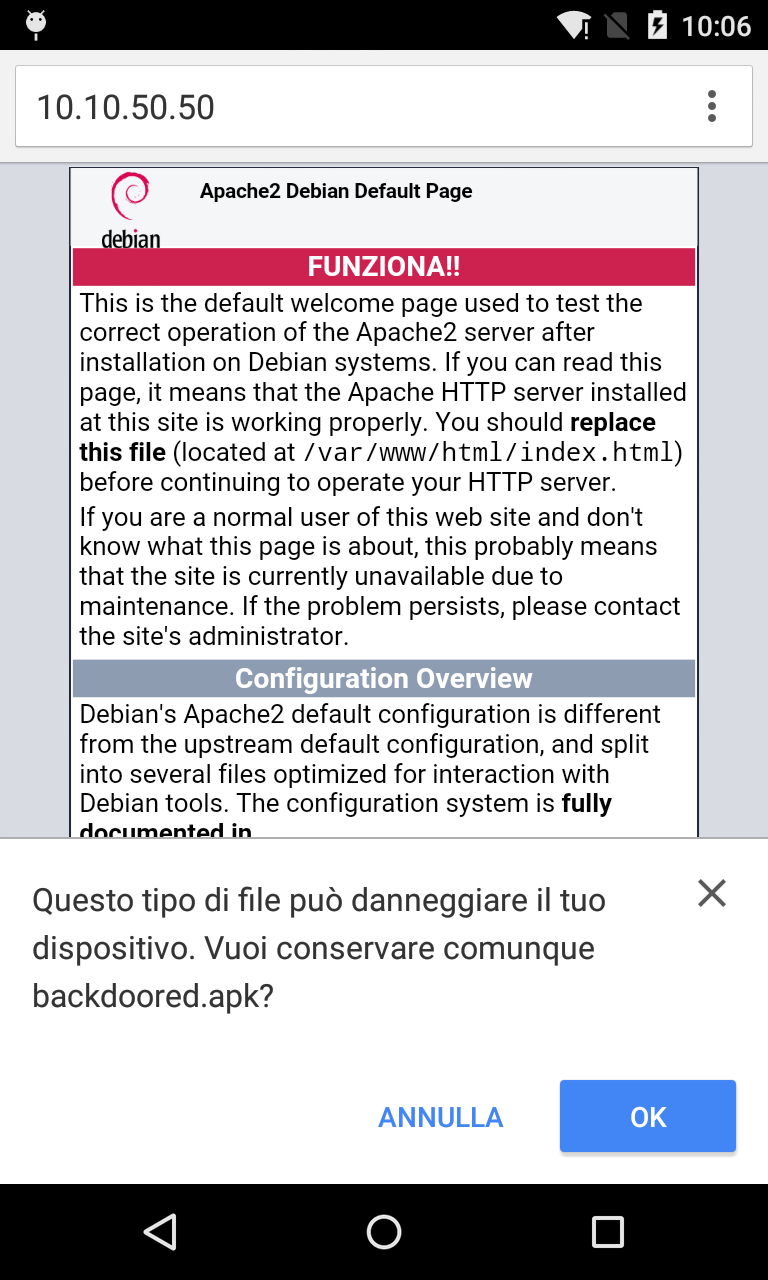
\includegraphics[width=.3\textwidth]{app/download}\label{fig:server}} \quad
		\subfloat[Installazione.]{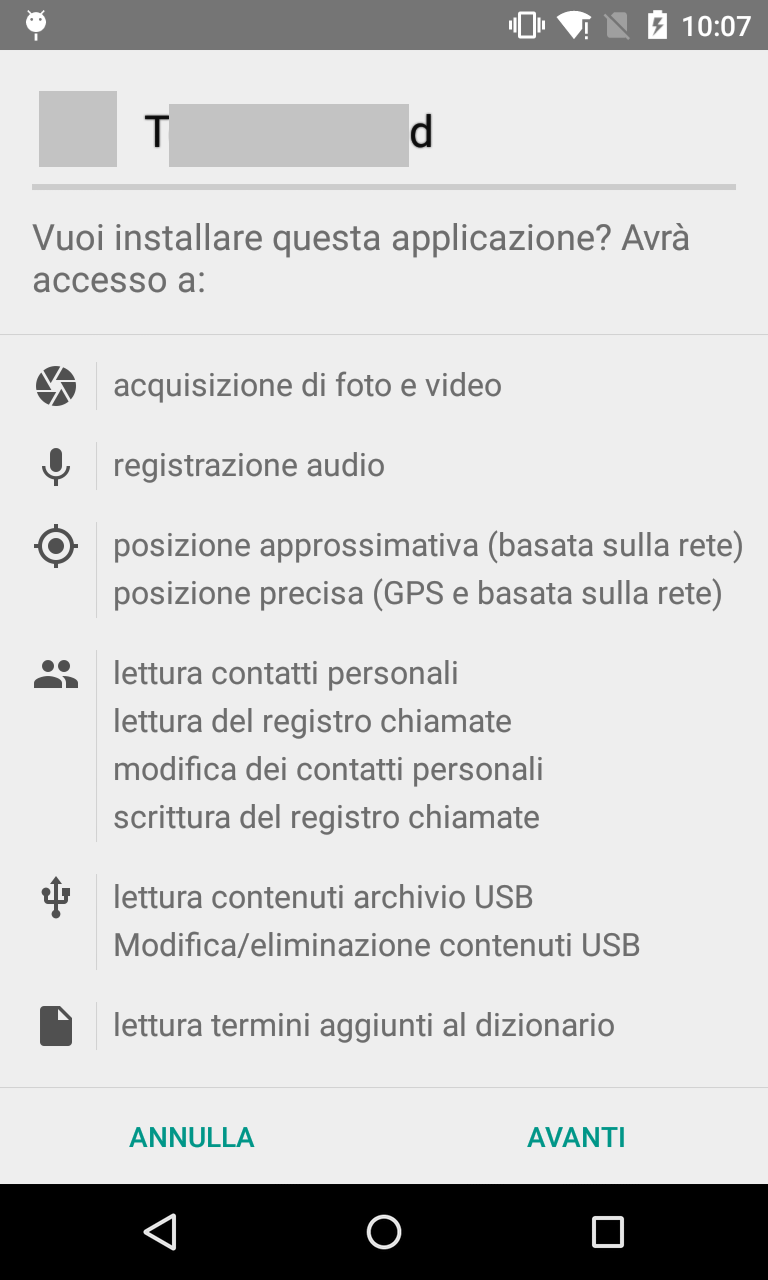
\includegraphics[width=.3\textwidth]{app/installazione}} \quad
		\subfloat[Applicazione.]{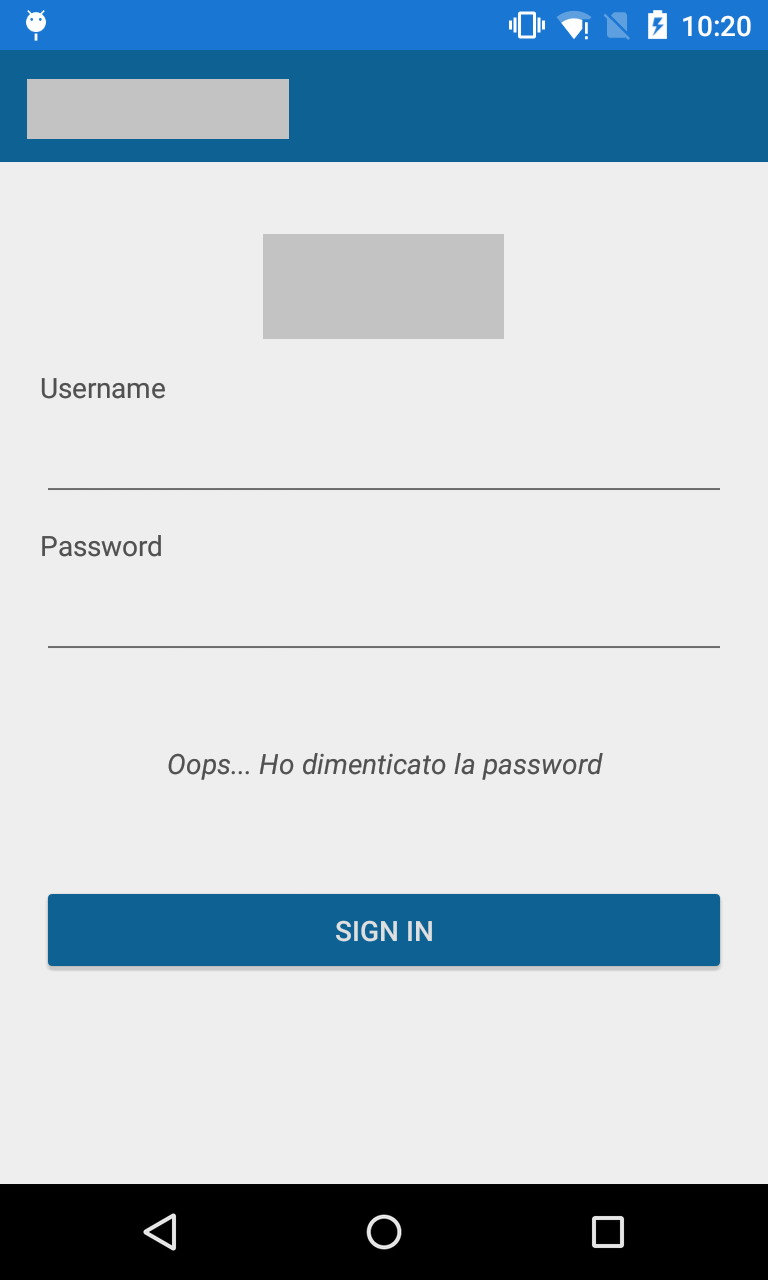
\includegraphics[width=.3\textwidth]{app/applicazione}\label{fig:grafica}}
	}
	\caption{Operazioni lato vittima.}
\end{figure}

Come si può vedere, l'applicazione installata è indistinguibile dall'originale sia come grafica (figura \ref{fig:grafica}) che come utilizzo in quanto non sono state apportate modifiche alle funzionalità della stessa. 

Nel momento in cui viene lanciata la prima volta, viene contattato il server \ac{CC} sulla porta $4444$, viene creata la connessione, si apre una sessione \emph{meterpreter} (figura \ref{fig:meterpreter}) e l'attaccante ha accesso al dispositivo vittima. Adesso è possibile scaricare l'elenco dei contatti, dei messaggi, delle foto e video, registrare audio, effettuare screenshot, scattare foto e registrare video tramite la fotocamera. Una volta ottenuto l'accesso al dispositivo è anche possibile installare in autonomia altre applicazioni malevole utili all'attaccante per aumentare il proprio potere di controllo sul dispositivo. Tutte queste operazioni vengono eseguite in maniera perfettamente trasparente alla vittima che non ha modo di accorgersi di quello che sta succedendo. 

È da notare il fatto che questa connessione sopravvive alla chiusura dell'applicazione e viene reinstaurata anche dopo un riavvio del dispositivo il quale risulta compromesso in maniera quasi irreversibile.

\begin{figure}[h]
	\centering
	\fbox{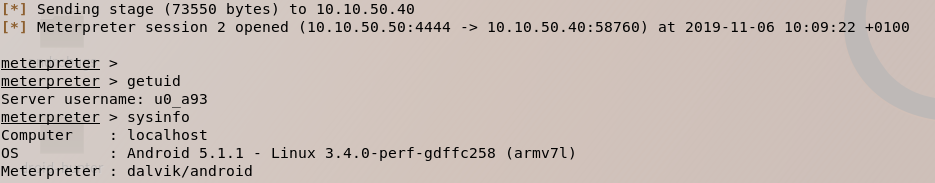
\includegraphics[width=.9\textwidth]{app/meterpreter}} 
	\caption{Connessione col server C\&C.}
	\label{fig:meterpreter} 
\end{figure}

\section{Soluzione}

Per quanto quella appena descritta non sia una vulnerabilità specifica dell'applicazione sotto analisi, è comunque importante rendere consapevole l'utente finale di questo rischio ed istruirlo a non installare mai applicazioni provenienti da sorgenti non sicure.

L'offuscamento del codice potrebbe rendere più difficile la decompilazione e la modifica dell'apk originale mitigando parzialmente questo tipo di problema ma la protezione totale è purtroppo impossibile da ottenere.
%-----------------APPENDICI------------------------------------
\appendix
\chapter{OWASP Mobile Top 10 risks}

	Si riporta la lista "Mobile top $10$ $2016$"\cite{OWASPtop10} stilata da OWASP Foundation:
	
	\begin{itemize}
		\item \textbf{M1 - Improper Platform Usage}; This category covers misuse of a platform feature or failure to use platform security controls. It might include Android intents, platform permissions, misuse of TouchID, the Keychain, or some other security control that is part of the mobile operating system. There are several ways that mobile apps can experience this risk.
		\item \textbf{M2 - Insecure Data Storage}; This new category is a combination of M2 + M4 from Mobile Top Ten 2014. This covers insecure data storage and unintended data leakage.
		\item \textbf{M3 - Insecure Communication}; This covers poor handshaking, incorrect SSL versions, weak negotiation, cleartext communication of sensitive assets, etc.
		\item \textbf{M4 - Insecure Authentication}; This category captures notions of authenticating the end user or bad session management. This can include:
		\begin{itemize}
			\item Failing to identify the user at all when that should be required
			\item Failure to maintain the user's identity when it is required
			\item Weaknesses in session management
		\end{itemize}		
		\item \textbf{M5 - Insufficient Cryptography}; The code applies cryptography to a sensitive information asset. However, the cryptography is insufficient in some way. Note that anything and everything related to TLS or SSL goes in M3. Also, if the app fails to use cryptography at all when it should, that probably belongs in M2. This category is for issues where cryptography was attempted, but it wasn't done correctly.
		\item \textbf{M6 - Insecure Authorization}; This is a category to capture any failures in authorization (e.g., authorization decisions in the client side, forced browsing, etc.). It is distinct from authentication issues (e.g., device enrolment, user identification, etc.). If the app does not authenticate users at all in a situation where it should (e.g., granting anonymous access to some resource or service when authenticated and authorized access is required), then that is an authentication failure not an authorization failure.
		\item \textbf{M7 - Client Code Quality}; This was the "Security Decisions Via Untrusted Inputs", one of our lesser-used categories. This would be the catch-all for code-level implementation problems in the mobile client. That's distinct from server-side coding mistakes. This would capture things like buffer overflows, format string vulnerabilities, and various other code-level mistakes where the solution is to rewrite some code that's running on the mobile device.
		\item \textbf{M8 - Code Tampering}; This category covers binary patching, local resource modification, method hooking, method swizzling, and dynamic memory modification. Once the application is delivered to the mobile device, the code and data resources are resident there. An attacker can either directly modify the code, change the contents of memory dynamically, change or replace the system APIs that the application uses, or modify the application's data and resources. This can provide the attacker a direct method of subverting the intended use of the software for personal or monetary gain.
		\item \textbf{M9 - Reverse Engineering}; This category includes analysis of the final core binary to determine its source code, libraries, algorithms, and other assets. Software such as IDA Pro, Hopper, otool, and other binary inspection tools give the attacker insight into the inner workings of the application. This may be used to exploit other nascent vulnerabilities in the application, as well as revealing information about back end servers, cryptographic constants and ciphers, and intellectual property.
		\item \textbf{M10 - Extraneous Functionality}; Often, developers include hidden backdoor functionality or other internal development security controls that are not intended to be released into a production environment. For example, a developer may accidentally include a password as a comment in a hybrid app. Another example includes disabling of 2-factor authentication during testing.
	\end{itemize} 
%-----------------BIBLIOGRAFIA---------------------------------
\bibliography{bib/bibliografia}
\bibliographystyle{unsrt}
%-----------------INDICI---------------------------------------
\addcontentsline{toc}{chapter}{Acronimi}

\chapter*{Acronimi}
	\begin{acronym}[CAGD]
		\acro{AES}{Advanced Encryption Standard}
		\acro{ARM}{Advanced RISC Machine}
		\acro{BP}{Branch Predictor}
		\acro{CNES}{Centre National d’Etudes Spatiales}
		\acro{CRT}{Chinese Remainder Theorem}
		\acro{CVE}{Common Vulnerabilities and Exposures}
		\acro{DBA}{Differential Behavior Analysis}
		\acro{DES}{Data Encryption Standard}
		\acro{DFA}{Differential Fault Analysis}
		\acro{DFIA}{Differential Fault Intensity Analysis}
		\acro{DH}{Diffie-Hellman}
		\acro{DPA}{Differential Power Analysis}
		\acro{DSA}{Digital Signature Algorithm}
		\acro{DSS}{Digital Signature Standard}
		\acro{FBA}{Fault Behavior Analysis}
		\acro{FIPS}{Federal Information Processing Standards}
		\acro{FSA}{Fault Sensitivity Analysis}
		\acro{GPS}{Global Positioning System}
		\acro{HTTPS}{HyperText Transfer Protocol over Secure Socket Layer}
		\acro{LED}{Light Emitting Diode}
		\acro{LLC}{Last Level Cache}
		\acro{NATO}{North Atlantic Treaty Organization}
		\acro{NCSCD4}{National Communications Security Committee Directive 4}
		\acro{NIST}{National Institute of Standards and Technology}
		\acro{PICA}{Picosecond Imaging Circuit Analysis}
		\acro{PoC}{Proof of Concept}
		\acro{QIF}{Quantitative Information-flow Analysis}
		\acro{SEA}{Safe-Error Attacks}
		\acro{SPA}{Simple Power Analysis}
		\acro{SPARK}{Spectre-based Password-avoiding Attack to Retrieve Keys}
		\acro{TEMPEST}{Transient Electromagnetic Pulse Emanation STandard}
		\acro{TOR}{The Onion Router}
	  	\acro{USB}{Universal Serial Bus}
	\end{acronym}
\end{document}